\documentclass[a4paper,11pt,titlepage]{scrbook}
\usepackage[utf8]{inputenc} %codificacion
\usepackage[spanish]{babel} %idioma

%\usepackage{titlesec}
%\usepackage{palatino} %usar fot palatino en vez de times roman

%\decimalpoint %revisar
%\usepackage{dcolumn} %revisat
%\newcolumntype{.}{D{.}{\esperiod}{-1}}
%\makeatletter
%\addto\shorthandsspanish{\let\esperiod\es@period@code}
%\makeatother


%\usepackage[chapter]{algorithm}
%\RequirePackage{verbatim}
%\RequirePackage[Glenn]{fncychap}
\usepackage{fancyhdr} %estilo del documento
\usepackage{graphicx} %colores
\usepackage{afterpage} %\clearpage y un par mas de funcs
\usepackage{longtable} %tabular and table extra opcs
\usepackage{xcolor}   %opcs colores
\definecolor{portada}{RGB}{239,206,53}
\definecolor{base}{RGB}{35,31,32}
\usepackage{pdfpages} %inclusion de archivos al doc
\usepackage[acronym]{glossaries} %acronimos y abreviaturas
\usepackage{acronym}
\usepackage{breakcites} %modifica \cite
\usepackage{natbib}

\renewcommand{\glossaryname}{Glosario}
\renewcommand{\acronymname}{Acrónimos}

%Instrucciones para poder escribir código y mostrarlo de manera elegante:
\definecolor{gray97}{gray}{.97}
\definecolor{gray75}{gray}{.75}
\definecolor{gray45}{gray}{.45}
\definecolor{gray30}{gray}{.94}

\usepackage{listings} %para escribir codigo
\lstset{ frame=Ltb,
framerule=0pt,
aboveskip=0.5cm,
framextopmargin=3pt,
framexbottommargin=3pt,
framexleftmargin=0.4cm,
framesep=0pt,
rulesep=.4pt,
backgroundcolor=\color{gray97},
rulesepcolor=\color{black},
%
stringstyle=\ttfamily,
showstringspaces = false,
basicstyle=\small\ttfamily,
commentstyle=\color{gray45},
keywordstyle=\bfseries,
%
numbers=left,
numbersep=15pt,
numberstyle=\tiny,
numberfirstline = false,
breaklines=true,
literate={á}{{\'a}}1 {Á}{{\'A}}1 {é}{{\'e}}1 {É}{{\'e}}1 {í}{{\'i}}1  {Í}{{\'I}}1  {ó}{{\'o}}1  {Ó}{{\'O}}1  {ú}{{\'u}}1  {Ú}{{\'U}}1  {Ñ}{{\~N}}1 {ñ}{{\~n}}1 ,
}



% minimizar fragmentado de listados
\lstnewenvironment{listing}[1][]
   {\lstset{#1}\pagebreak[0]}{\pagebreak[0]}

\lstdefinestyle{Consola}
   {basicstyle=\scriptsize\bf\ttfamily,
    backgroundcolor=\color{gray30},
    frame=single,
    numbers=none
   }
\lstdefinestyle{C}
	{basicstyle=\scriptsize,
	frame=single,
	language=C,
	numbers=left
	}
\lstdefinestyle{CodigoC++}
        {basicstyle=\small,
	frame=single,
	backgroundcolor=\color{gray30},
	language=C++,
	numbers=left
 	}
\lstdefinestyle{PHP}
	{basicstyle=\scriptsize,
%        {basicstyle=\small,
	frame=single,
	language=PHP,
	numbers=left
	}
	
%OPCS PROPIAS
\setlength{\parskip}{.8em}
\newcommand\placeholdertext[1]{\fcolorbox{black}{yellow}
{\textcolor{red}{#1}}}

%


% ********************************************************************
% Información sobre el TFG. Comentar lo que NO se desee añadir y sustituir con la información correcta.
% ********************************************************************
\newcommand{\myTitle}{Gestión y manejo de comportamientos grupales 
de entidades en videojuegos}
\newcommand{\mySubtitle}{\placeholdertext{Subtítulo del TFG}}
\newcommand{\myDegree}{Grado en Ingeniería Multimedia}
\newcommand{\myName}{Borja Pozo Wals}
\newcommand{\myProf}{Francisco José Gallego Durán}
%\newcommand{\myOtherProf}{Nombre Apellido1 Apellido2 (tutor2)}
\newcommand{\myFaculty}{Escuela Politécnica Superior de la Universidad de Alicante}
\newcommand{\myFacultyShort}{EPS UA}
\newcommand{\depTutorOne}{Departamento de Ciencia de la Computación e Inteligencia Artificial}
%\newcommand{\depTutorTwo}{Departamento del cotutor}


\newcommand{\myUni}{\protect{Universidad de Alicante}}
\newcommand{\myLocation}{Alicante}
\newcommand{\myTime}{\today}
%\newcommand{\myVersion}{Version 0.1}

\newcommand{\logoGrado}{imagenes/logoim.jpg}
\newcommand{\logoFacultad}{imagenes/logoeps.jpg}
\newcommand{\logoUniversidad}{imagenes/logoua.jpg}

\usepackage{url}

% Definición de comandos que me son útiles:
%\renewcommand{\indexname}{Índice alfabético}
%\renewcommand{\glossaryname}{Glosario}

\pagestyle{fancy}
\fancyhf{}
\fancyhead[LO]{\leftmark}
\fancyhead[RE]{\rightmark}
\fancyhead[RO,LE]{\textbf{\thepage}}
\renewcommand{\chaptermark}[1]{\markboth{\textbf{#1}}{}}
\renewcommand{\sectionmark}[1]{\markright{\textbf{\thesection. #1}}}


\setlength{\headheight}{1.5\headheight}

\newcommand{\HRule}{\rule{\linewidth}{0.5mm}}
%Definimos los tipos teorema, ejemplo y definición podremos usar estos tipos
%simplemente poniendo \begin{teorema} \end{teorema} ...
\newtheorem{teorema}{Teorema}[chapter]
\newtheorem{ejemplo}{Ejemplo}[chapter]
\newtheorem{definicion}{Definición}[chapter]
 
\newcommand{\bigrule}{\titlerule[0.5mm]}


%Para conseguir que en las páginas en blanco no ponga cabeceras
\makeatletter
\def\clearpage{%
  \ifvmode
    \ifnum \@dbltopnum =\m@ne
      \ifdim \pagetotal <\topskip
        \hbox{}
      \fi
    \fi
  \fi
  \newpage
  \thispagestyle{empty}
  \write\m@ne{}
  \vbox{}
  \penalty -\@Mi
}
\makeatother

\usepackage[pdfborder={000}]{hyperref} %referencia
\hypersetup{
pdfauthor = {\myName (bpw1@alu.ua.es)},
pdftitle = {\myTitle},
pdfsubject = {},
pdfkeywords = {AI, Inteligencia Artificial, Videojuegos, C++},
pdfcreator = {LaTeX con el paquete ....},
pdfproducer = {pdflatex}
}
%AQUI COMIENZA LA LISTA DE FICHEROS A INCLUIR


\begin{document}
\renewcommand{\listtablename}{Índice de tablas} %para sustituir la palabra cuadro por tabla
\renewcommand{\tablename}{Tabla}
\renewcommand{\lstlistingname}{Listado}
\renewcommand{\lstlistlistingname}{Índice de \lstlistingname s}

\frontmatter
\begin{titlepage}

\newlength{\centeroffset}
\setlength{\centeroffset}{-0.5\oddsidemargin}
\addtolength{\centeroffset}{0.5\evensidemargin}
\thispagestyle{empty}

\includepdf[pages={1},pagecommand={},fitpaper=true,trim=0 0 0 0, 
offset=0 0,turn=true,noautoscale=true]{portada/portada.pdf}

\end{titlepage}
\pagecolor{white} %la portada en color
\begin{titlepage}
 
 
\setlength{\centeroffset}{-0.5\oddsidemargin}
\addtolength{\centeroffset}{0.5\evensidemargin}
\thispagestyle{empty}

\noindent\hspace*{\centeroffset}\begin{minipage}{\textwidth}

\centering


% Title

%{\Huge\bfseries Título del proyecto\\ }
{\Huge\bfseries \myTitle}

\noindent\rule[-1ex]{\textwidth}{3pt}\\[3.5ex]
{\large\bfseries \mySubtitle\\[4cm]}
\end{minipage}

\vspace{2.5cm}
\noindent\hspace*{\centeroffset}\begin{minipage}{\textwidth}
\centering

\textbf{Autor}\\ {\myName}\\[2.5ex]
\textbf{Tutor/es}\\
{\normalsize \myProf\\
\small\textit \depTutorOne\\[6cm]}
%\normalsize \myOtherProf\\
%\small\textit \depTutorTwo

\includegraphics[scale=0.75]{\logoGrado}


\textsc{\myDegree}\\[4mm]

\centering
\begin{minipage}[l]{7cm}
\includegraphics[width=5cm]{\logoFacultad}
\end{minipage}
\begin{minipage}[r]{7cm}
\hspace{1cm}
\includegraphics[width=5cm]{\logoUniversidad}
\end{minipage}\\[0.4cm]


%\textsc{\myFaculty}\\

%\large\bfseries \textsc{\myUni}\\
ALICANTE, \myTime

\end{minipage}
%\addtolength{\textwidth}{\centeroffset}
\vspace{\stretch{2}}

\end{titlepage}


 %la portada en b/n
%\chapter*{Preámbulo}
\thispagestyle{empty}
\textbf{titulo por definir} es una herramienta para simular escenarios 
 bélicos como los que podemos encontrar en juegos del género \ac{RTS} como son
 `Mount \& Blade' o la saga `Imperium', desarrollado completamente en C++ para \ac{PC}.

La simulación se compone de un escenario, una unidad controlada por el jugador,
una serie de unidades que conforman el ejercito bajo sus ordenes y por último, 
tenemos una serie de objetivos que abatir. Una vez conseguido el objetivo terminará
el juego pudiendo el jugador elegir entre repetir el nivel o volver al menú principal.


\cleardoublepage %salta a nueva página impar
\chapter*{Agradecimientos\footnote{Por si alguien tiene curiosidad, este ``simpático'' agradecimiento está tomado de la ``Tesis de Lydia Chalmers'' basada en el universo del programa de televisión Buffy, la Cazadora de Vampiros.http://www.buffy-cazavampiros.com/Spiketesis/tesis.inicio.htm}
}

\thispagestyle{empty}
\vspace{1cm}

Este trabajo no habría sido posible sin el apoyo y el estimulo de mi colega y amigo, Doctor Rudolf Fliesning,  bajo cuya supervisión escogí este tema y comencé la tesis. Sr. Quentin Travers, mi consejero en las etapas finales del trabajo, también ha sido generosamente servicial, y me ha ayudado de numerosos modos, incluyendo el resumen del contenido de los documentos que no estaban disponibles para mi examen, y en particular por permitirme leer, en cuanto estuvieron  disponibles, las copias de los  recientes extractos de los diarios de campaña del Vigilante Rupert Giles y la actual Cazadora la señorita Buffy Summers, que se encontraron con William the Bloody en 1998, y por facilitarme el pleno acceso  a los diarios de anteriores Vigilantes relevantes a la carrera de William the Bloody.

También me gustaría agradecerle al Consejo la concesión de Wyndham-Pryce como Compañero, el cual me ha apoyado durante mis dos años de investigación, y la concesión de dos subvenciones de viajes, una para estudiar documentos en los Archivos de Vigilantes sellados en Munich, y otra para la investigación en campaña en Praga. Me gustaría agradecer a Sr. Travers, otra vez, por facilitarme  la acreditación  de seguridad para el trabajo en los Archivos de Munich, y al Doctor Fliesning por su apoyo colegial y ayuda en ambos viajes de investigación.

No puedo terminar sin agradecer a mi familia, en cuyo estímulo constante y amor he confiado a lo largo de mis años en la Academia. Estoy agradecida también a los ejemplos de mis  difuntos hermano, Desmond Chalmers, Vigilante en Entrenamiento, y padre, Albert Chalmers, Vigilante. Su coraje resuelto y convicción siempre me inspirarán, y espero seguir, a mi propio y pequeño modo, la noble misión por la que dieron sus vidas. 

Es a ellos a quien dedico este trabajo.

\cleardoublepage %salta a nueva página impar
% Aquí va la dedicatoria si la hubiese. Si no, comentar la(s) linea(s) siguientes
\chapter*{}
\setlength{\leftmargin}{0.5\textwidth}
\setlength{\parsep}{0cm}
\addtolength{\topsep}{0.5cm}
\begin{flushright}
\small\em{
A mi esposa Marganit, y a mis hijos Ella Rose y Daniel Adams,\\
sin los cuales habría podido acabar este libro dos años antes \footnote{Dedicatoria de Joseph J. Roman en "An Introduction to Algebraic Topology"}
}
\end{flushright}


\cleardoublepage %salta a nueva página impar
% Aquí va la cita célebre si la hubiese. Si no, comentar la(s) linea(s) siguientes
\chapter*{}
\setlength{\leftmargin}{0.5\textwidth}
\setlength{\parsep}{0cm}
\addtolength{\topsep}{0.5cm}
\begin{flushright}
\small\em{
Si consigo ver más lejos\\
es porque he conseguido auparme\\ 
a hombros de gigantes
}
\end{flushright}
\begin{flushright}
\small{
Isaac Newton.
}
\end{flushright}
\cleardoublepage %salta a nueva página impar

\chapter*{Resumen}
\label{Resumen}
%\thispagestyle{empty}
\textbf{titulo por definir} es una herramienta para simular escenarios 
 bélicos como los que podemos encontrar en juegos del género \ac{RTS} como son
 `Mount \& Blade' o la saga `Imperium', desarrollado completamente en C++ para \ac{PC}.

La simulación se compone de un escenario, una unidad controlada por el jugador,
una serie de unidades que conforman el ejercito bajo sus ordenes y por último, 
tenemos una serie de objetivos que abatir. Una vez conseguido el objetivo terminará
el juego pudiendo el jugador elegir entre repetir el nivel o volver al menú principal.

\chapter*{Justificación y objetivos}
A lo largo de la carrera son muchas las asignaturas que requieren y desarrollan
habilidades relacionadas con la programación en diversos lenguajes y usos, 
pero no es hasta el tercer año que se me presenta la oportunidad de desarrollar
un videojuego completo. 

Durante la asignatura de `Fundamentos de los Videojuegos' tuve por primera vez
la experiencia de enfrentarme al desafio que es crear un videojuego, y fue en ese
momento cuando me di cuenta de que a lo que me quería dedicar es a
desarrollar juegos de forma profesional. A lo largo del cuarto curso junto a los demás
integrantes de \textit{'Sunlight Studio'} desarrollamos \textit{'Cyborgeddon'}, y fue
en este momento que terminé de decidir que es a lo quiero dedicarme en el futuro.

A lo largo de mi vida he jugando una considerable cantidad de juegos entre los cuales
se puede apreciar una inclinación por los juegos de aventura y exploración, los 
\ac{RPG} y los \ac{RTS} o de estrategia en general, es por esto que me hace especial
ilusión desarrollar un juego de uno de estos géneros.\\
Teniendo en cuenta esto la elección de desarrollar un juego del tipo \ac{RTS} para la
realización del \ac{TFG} se debe a que según mi criterio es el que tiene mayor
potencial para ayudarme a mejorar mis habilidades como programador, ya que se basa en
unas mecánicas con las que no he trabajado con anterioridad.

Una vez dicho esto, los objetivos planteados para el proyecto son los siguientes:
\begin{itemize}
	\item Aumentar mis conocimientos de C++
	\item Comprender mejor el funcionamiento del \ac{PC}
	\item Aprender nuevas técnicas de \ac{IA}
	\item Desarrollar un producto mediante el cual mostrar mis habilidades
\end{itemize}

\cleardoublepage %salta a nueva página impar
% Aquí va la dedicatoria si la hubiese. Si no, comentar la(s) linea(s) siguientes
\chapter*{Agradecimientos}
\setlength{\leftmargin}{0.5\textwidth}
\setlength{\parsep}{0cm}
\addtolength{\topsep}{0.5cm}
\begin{flushright}
\small\em{
A mi madre Gabriela,\\
por el increíble esfuerzo que realiza cada día por mi. 
}
\end{flushright}
\begin{flushright}
\small\em{
A mi hermana Raquel,\\
por haber sido y ser un faro para mi. 
}
\end{flushright}
\begin{flushright}
\small\em{
A mi buen compañero Jorge Espinosa,\\
por nuestra convivencia estos años. 
}
\end{flushright}
\begin{flushright}
\small\em{
A mi querido amigo Guillermo y su familia,\\
por el cariño recibido incluso a pesar de la distancia. 
}
\end{flushright}

\cleardoublepage %salta a nueva página impar
% Aquí va la cita célebre si la hubiese. Si no, comentar la(s) linea(s) siguientes
\chapter*{}
\setlength{\leftmargin}{0.5\textwidth}
\setlength{\parsep}{0cm}
\addtolength{\topsep}{0.5cm}
\begin{flushright}
\small\em{
Ni los reyes ni los gobernantes llevan el cetro,\\
sino los que saben mandar\\ 
}
\end{flushright}
\begin{flushright}
\small{
Sócrates.
}
\end{flushright}

\begin{flushright}
\small\em{
Para saber hablar es preciso saber escuchar\\
}
\end{flushright}
\begin{flushright}
\small{
Plutarco.
}
\end{flushright}
\cleardoublepage %salta a nueva página impar
 %editar este texto (capitulos/preliminares.tex) para cambiar preámbulo, agradecimientos y dedicatorias
\tableofcontents
\listoffigures
\listoftables
\lstlistoflistings
\chapter*{Índice de Acrónimos}
\label{acronimos}
% fichero para poner los acrónimos
%para escribir un acrónimo nuevo, seguir el siguiente protocolo: (POR EJEMPLO PARA PONER EL ACRÓNIMO IEEE)
%- En el texto, poned \ac{IEEE}
%- En el fichero acrónimos.tex, poner la siguiente enTrada:
% \acrodef{IEEE}{Institute of Electrical and Electronics Engineers}
% IEEE: Institute of Electrical and Electronics Engineers

%Además de \ac{IEEE} se pueden usar otras fórmulas en el texto para variar el comportamiento del paquete de acrónimos:
% Por ejemplo:
% acf{} hace que siempre aparezca el texto completo del acrónimo correspondiente. (fórmula larga y corta)
% acl{} hace que Solo aparezca la fórmula larga
% acs{} hace que aparezca obligatoriamente la fórmula corta
% acp{} incluye el plural del acrónimo.
% acs{} hace que aparezca la versión córta del acrónimo.
% acresetall{} resetea todos los acrónimos de forma que se establecen como “no usados”.
% acused{} marca el acrónimo como “usado”.

A lo largo del documento serán utilizadas una serie de abreviaturas con el fin de
hacer más cómoda su lectura. Todos los términos están indicados a continuación: 

\begin{itemize}

\acrodef{TFG}{Trabajo Final de Grado}
\acrodefplural{TFG}[TFG]{Trabajos Finales de Grado}
\item \textbf{TFG:} Trabajo Final de Grado

\acrodef{PC}{Personal Computer}
\acrodefplural{PC}[PC]{Personal Computers}
\item \textbf{PC:} Personal Computer

\acrodef{RTS}{Real Time Strategy}
\item \textbf{RTS:} Real Time Strategy

\acrodef{RPG}{Rol Play Game}
\acrodefplural{RPG}[RPG]{Rol Play Games}
\item \textbf{RPG:} Rol Play Game

\acrodef{IA}{Inteligencia Artificial}
\acrodefplural{IA}[IA]{Inteligencias Artificiales}
\item \textbf{IA:} Inteligencia Artificial

\acrodef{NPC}{Non-Player Character}
\acrodefplural{NPC}[NPC]{Non-Player Characters}
\item \textbf{NPC:} Non-Player Character

\acrodef{AoE}{Age of Empires}
\acrodefplural{AoE}[AoE]{Age of Empires}
\item \textbf{AoE:} Age of Empires

\acrodef{TaB}{They are Billions}
\acrodefplural{TaB}[TaB]{They are Billions}
\item \textbf{TaB:} They are Billions

%borrar
\acrodef{TFM}{Trabajo Final de Master}
\acrodef{IEEE}{Institute of Electrical and Electronics Engineers}
\acrodef{EPS}{Escuela Politécnica Superior} 
\acrodef{APA}{American Psychological Association}

\end{itemize}

\mainmatter %entre frontmatter y mainmatter, la numeración es en romanos.

%a continuación se propone un esquema de trabajo que puede ser alterado justificadamente.
\acresetall{}  % resetea los acrónimos por si han sido usados en el índice o en los preliminares.
\chapter{Introducción}
\label{intro}
Este proyecto trata sobre el desarrollo de un simulador de batallas para \ac{PC}
desarrollado en \textit{Linux}, escrito en C++ y haciendo uso de librerias escritas en
C como TinyPTC *add reference*.

El simulador, \textbf{inserte título}, se trata de una demo del género \ac{RTS}
compuesta por un escenario a través del cual tendremos que comandar y luchar junto a
nuestro ejercito con el fin de abatir al ejercito rival. El escenario estará compuesto
por estructuras y obstáculos que deberemos sortear para alcanzar nuestro objetivo.

A nivel técnico el proyecto cuenta con el desafio de desarrollar una \ac{IA} grupal
para los \ac{NPC} basada en el uso de técnicas como los \textit{Steering behaviours} 
y el \textit{Flocking} con el fin de emular un comportamiento coordinado entre las
distintas entidades. El objetivo es crear una versión inicial sencilla mediante la 
cual poder profundizar en los conceptos en los cuales se basan las mencionadas técnicas
con el fin de desarrollar una versión más compleja y específica para nuestro proyecto
de forma que se adapte de la mejor forma posible a nuestras necesidades.

Por otro lado, como objetivo adicional fuera de la demo como tal es realizar
un \textit{port} a \textit{Windows} con el fin de poder mostrar los resultados
en ambos sistemas operativos.




\chapter{Marco teórico}
\label{Marco_teorico}

\section{Estudio de mercado}
A lo largo de los años los \ac{RTS} siempre han contado con una gran aceptación entre
los usuarios de \ac{PC}, un claro ejemplo de esto puede ser el juego \textit{`Age of
Empire II: The Age of Kings'}\footnote{Desarrollado por `Ensemble Studios' y lanzado a
finales de 1999.} el cual se posicionó como uno de los juegos más vendidos del momento
superando el millón de copias. Actualmente el juego cuenta con una remasterización
\footnote{Co-desarrollado por Forgotten Empires, Tantalus Media y Wicked
Witch. Lanzado en noviembre de 2019.} la cual ha conseguido vender más de 50.000
copias en \textit{`Steam'}. Datos extraídos de su articulo en \citeauthor*{Wiki_AoE2}.

Si miramos en el panoráma nacional actual, podemos encontar el juego \textit{`They Are
Billions'} \footnote{Desarollado por Numantian Games y lanzado en junio de 2019.}
disponible inicialmente para \ac{PC} y posteriormente lanzado en \textit{`PlayStation 4'}
y \textit{`Xbox One'} debido a su éxito. A día de hoy el juego a conseguido vender
solamente en \textit{`Steam'} más de 25.000 unidades consiguiendo una valoración muy
positiva por parte de los usuarios de la plaforma como podemos ver en la página 
del juego de \citeauthor*{TaB2019} en dicha tienda.

El género puede aparentar ser cosa del pasado pero vistas las cifras podemos concluir
que sigue siendo un reclamo para los jugadores.

\section{Referentes}
A la hora de establecer las mecánicas, el estilo artístico y/o otros aparatados del
juego es habitual basarse o tener en cuenta lo que han hecho otras entregas anteriores
en su momento. Para el desarrollo de este proyecto han sido de gran utilidad una
serie de entregas entre las que cabe destacar dos.

\subsection{Age of Empires II: The Age of Kings}
En primer lugar encontramos el juego \textit{'Age of Empires II: The Age of Kings'}, en
este juego tendremos que gestionar una civilizacion a elegir entre un amplio abanico de
facciones con sus propias unidades y edificaciones.

\begin{figure}[ht]
\centering
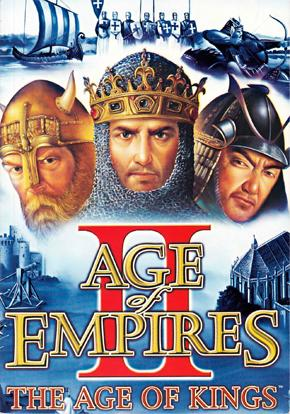
\includegraphics[width=0.3\textwidth]{imagenes/marco_teo/referentes/aoe_1.png}
\caption{Carátula del juego original.}
\label{img:aoe_1}
\end{figure}

El jugador deberá ser capaz de guiar a las unidades, gestionar las ciudades y conseguir
recursos a lo largo del escenario con el fin de derrotar a las demás facciones. Además,
se nos presenta una serie de campañas en las cuales manejaremos a grandes personajes de
la historia como `William Wallace' o `Juana de Arco' entre otros.

El juego hace de referente en varios aspectos entre los que podemos encontrar el
apartado visual donde se utiliza una perspectiva isométrica con cámara fija y el uso
de una estética clásica propia de las épocas a las que pertenecen las civilizaciones.

\begin{figure}[ht]
\centering
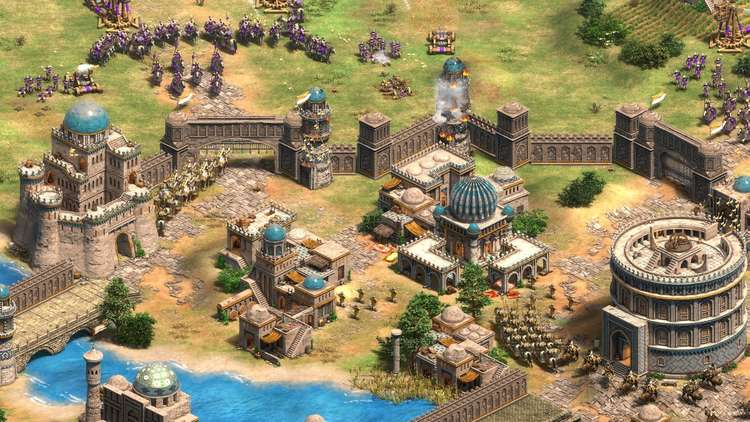
\includegraphics[width=0.7\textwidth]{imagenes/marco_teo/referentes/aoe_2.png}
\caption{Ciudad siendo asediada.}
\label{img:aoe_2}
\end{figure}

Todas la unidades de las que podemos disponer cuentan con una serie características que
las hacen más o menos fuertes en función del objetivo al que ataquen, podemos encontrar
el ejemplo de las máquinas de asedio las cuales son más fuertes contra estructuras pero
más débiles contra infanteria, o las unidades a caballo que son fuertes contra arqueros
e infanteria pero débiles frente a lanceros.
Este tipo de mécanicas dotan al juego de una importante componente táctica en el manejo
de las unidades que debemos dominar si queremos completar los diferentes niveles de
forma satisfactoria~\ref{img:aoe_2}.

\subsection{The Are Billions}
En segundo lugar podemos encontrar el juego \textit{'\acf{TaB}'} el cual reutiliza
una serie de características propias del género y como pueden ser la perspectiva
isométrica pero sin dejar de innovar introduciendo nuevas mecánicas y/o formas de
plantear la jugabilidad.

\begin{figure}[ht]
\centering

\includegraphics[width=0.7\textwidth]{imagenes/marco_teo/referentes/tab_1.png}
\caption{Imágen promocional del juego.}
\label{img:tab_1}
\end{figure}
 
En \textit{'\ac{TaB}'} podemos encontrar funciones interesantes como la pausa
táctica la cual nos permitirá visualizar detenidamente el estado del mapa sin tener que
preocuparnos por no estar atendiendo algunos posibles eventos como ataques a nuestras
tropas por parte del enemigo. En juegos anteriores como los \textit{'\ac{AoE}'} es
fácil encontrarnos en la situación de tener trabajadores en la ciudad sin hacer tareas
un rato y no poder mirar cuales son e ir pensando su ocupación siguiente por estar
atrapado en refriegas con otros jugadores, con este tipo de mecánicas estas situaciones
se solventan en mayor o menor medida y permiten al jugador tomarse el tiempo que
necesite para pensar las acciones que quiere realizar.

Otro aspecto llamativo en el podemos fijarnos es en la aparición de solamente dos
facciones. Por un lado encontramos `El Nuevo Imperio', la facción del jugador, la
cual representa una serie de colonias que tendremos que desarrollar a lo largo de
los niveles. En el otro lado encontramos las infinitas hordas de zombis que tratarán
de exterminar a la raza humana.

\begin{figure}[ht]
\centering
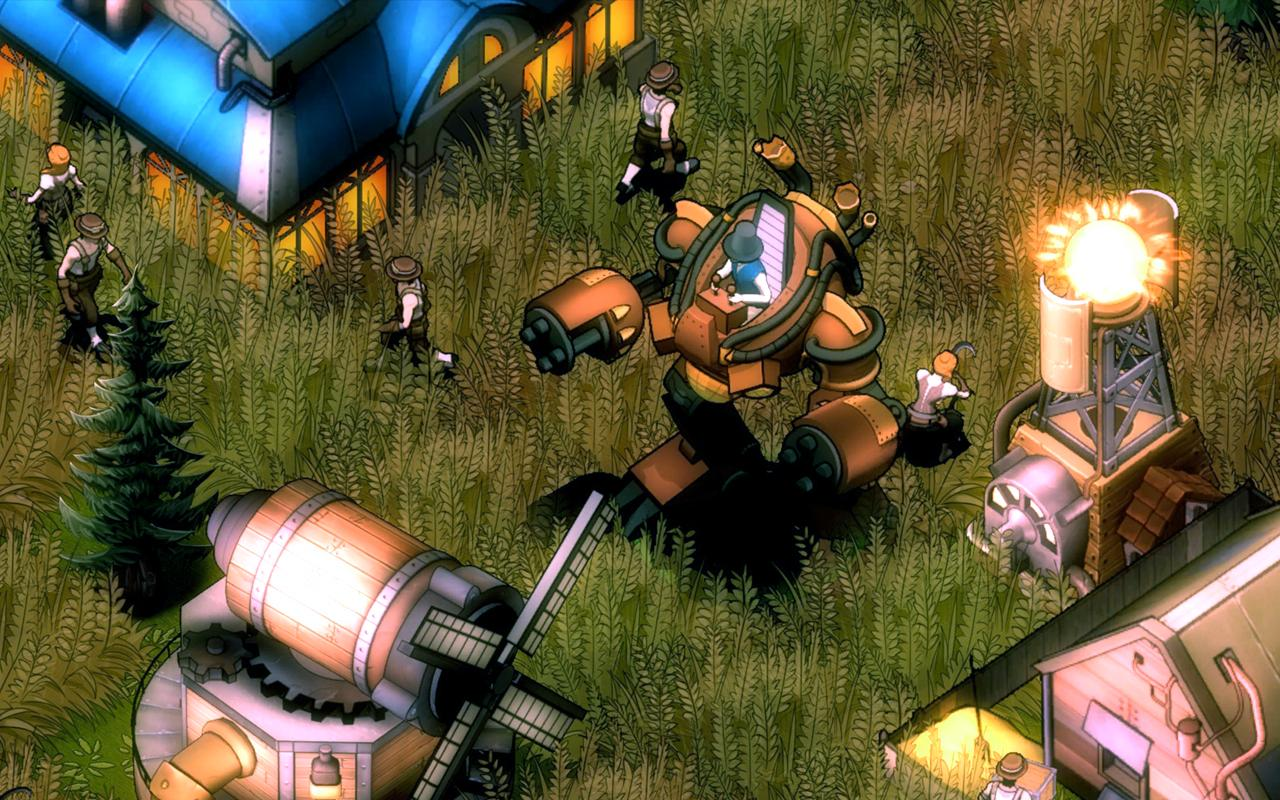
\includegraphics[width=0.6\textwidth]{imagenes/marco_teo/referentes/tab_2.png}
\caption{Ejemplo de unidad mecánica del imperio y estética del juego}
\label{img:tab_2}
\end{figure}

A diferencia de en \textit{'\ac{AoE}'} que todas la facciones poseen las mismas unidades
\footnote{Algunos valores pueden variar según bonos de facción}, en
\textit{'\ac{TaB}'} cada facción dispondrá de unidades únicas con acciones propias.
Como podemos ver en la imágen~\ref{img:tab_2} las tropas del imperio se basan en el uso
de maquinaria y armas de fuego para repeler las hordas enemigas, por otro lado los
zombis contarán con diversas caraterísticas físicas mejoradas conforme sean de mayor
``nivel'' puediendo encontrar algunos más rápidos, o más fuertes o más grandes y
resistentes al daño.~\ref{img:tab_3}

\begin{figure}[ht]
\centering

\includegraphics[width=0.5\textwidth]{imagenes/marco_teo/referentes/tab_3.png}
\caption{Infectado gigante}
\label{img:tab_3}
\end{figure}

Como último punto a destacar de la entrega tenemos la introducción del un modo de
juego de supervivencia donde a lo largo del tiempo irán apareciendo oleadas de zombis
donde cada vez aparecen más enemigos y más poderosos de forma infinita, haciendo así
que la partida termine cuando el jugador deje de aguantar la ofensiva enemiga.


\section{Técnicas de inteligencia articificial}
Como ya se ha mencionado anteriormente en la introducción~\ref{intro} de este \ac{TFG}
el grueso del desarrollo y uno de los objetivos más importantes del proyecto recaen en
el desarrollo de una \ac{IA} haciendo uso de las técnicas de \textit{'Flocking'} y
\textit{`Steering behaviors'}.

Para ello nos basaremos principalmente en las explicaciones y ejemplos que podemos
encontrar en el libro \cite[ch.~3]{Millington2009} donde de forma extensa y detallada
se nos introduce en la teoría relacionada a los algoritmos y la forma en la que estos
se estructuran e interactuan entre ellos. Para dar un poco de contexto sobre el tema
resumiremos brevemente las ideas que se nos presentan a lo largo del capitulo dedicado
a estas técnicas. 

Los \textit{`Steering behaviors'} pueden ser entendidos como una serie de algoritmos
destinados a guiar la forma en la cual los \ac{NPC} se desplazan por el escenario
y/o interactuan con los distintos elementos que puedan encontrase en la escena. Siguen
una filosofía de crear movimientos complejos a base de una combinación de movimientos 
y/o acciones simples, un ejemplo común puede ser la acción de perseguir a un objetivo
mientras se sortean obstáculos en el proceso. \\ 
En este caso no tendríamos una función llamada 
\textit{``persigue-enemigo-mientras-esquivas()''} y esta encargarse de todo el 
trabajo, sino que, tendremos el cálculo de la velocidad y dirección necesarias para
alcanzar el objetivo, la compropación para saber si hay algún tipo de
obstáculo por el camino y la rectificación de la trayectoria en caso de
haberlos cada uno por su lado y es la resultante de todos los pasos la que defina el
movimiento final.

Esta forma de estructurar y formar actividades complejas en base a acciones más simples
nos permite reutilizar y jugar con los diferentes comportamientos permitiéndonos crear
con ellos un amplio espectro de resultados.

En lo referente al \textit{'Flocking'} podemos observar como en esencia es lo mismo que
los \textit{`Steering behaviors'} pero añadiendo factores y/o componentes grupales,
el origen del modelo lo podemos encontrar en las publicaciones de \cite{Boids1986} donde
se nos introduce el concepto de \textit{``Boid''} como entidad generica que simula su
comportamiento bajo este algoritmo. Además, se nos introducen los tres comportamientos
básicos en los que se basa la técnica para generar el movimiento emergente, que son:

La \textbf{separación}~\ref{img:separation-b} que cada \textit{Boid} mantendrá entre
las demás entidades en su vencidad, con esto evitaremos solapamientos y respetar el
espacio y movimiento de las demás entidades.

\begin{figure}[ht]
\centering
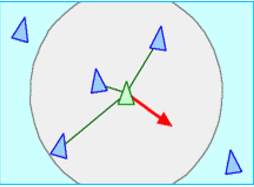
\includegraphics[width=0.35\textwidth]{imagenes/marco_teo/separation.png}
\caption{Separation behavior}
\label{img:separation-b}
\end{figure}

Por otro lado podemos encontrar el \textbf{alineamiento}~\ref{img:alignment-b} de la
dirección del movimento propio con las de las entidades más cercanas, de esta forma conseguimos un
movimiento armónico entre los \textit{boids} y produciremos una sensación de
coordinación entre ellos.

\begin{figure}[ht]
\centering
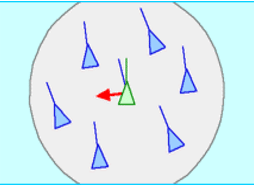
\includegraphics[width=0.35\textwidth]{imagenes/marco_teo/alignment.png}
\caption{Alignment behavior}
\label{img:alignment-b}
\end{figure}

Por último encontramos la \textbf{cohesión}~\ref{img:cohesion-b} la cual se encargará de
mantener a las entidades cercanas juntas para crear esa sensación de grupo que buscamos
con el algoritmo.

\begin{figure}[ht]
\centering
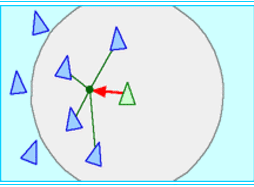
\includegraphics[width=0.35\textwidth]{imagenes/marco_teo/cohesion.png}
\caption{Cohesion behavior}
\label{img:cohesion-b}
\end{figure}

Por otro lado, podemos ver en el articulo de `Raynolds' como a lo largo de los años se
ha ido modificando y ampliando el algoritmo con el fin de añadir variaciones en el
comportamiento y/o introducir más factores influyentes en la decisión de los 
\textit{Boids} como puede ser el olor de determinada entidad/es y/o escenario. \\
Esto sin duda es gracias a la versatílidad que nos proporciona el uso de los
\textit{`Steering behaviors'} y jugar con la importancia de las distintas componentes
a la hora de hacer la toma de decisiones.


\chapter{Documento de Diseño del Juego (GDD)}
\label{GDD}

\section{Descripción general}
El juego que se pretende desarrollar se basa en el apartado de navegación por el mapa y combate
típicos en los \ac{RTS}. A lo largo de los distintos niveles, el jugador deberá hacer
frente a distintos desafíos como pueden ser: escoltar con sus unidades de un punto
del mapa a otro a un personaje importante y/o eliminar a todas las entidades enemigas del escenario.

\section{Mecánicas}
Durante el juego podremos ejecutar una serie de ordenes sobre nuestras unidades para cambiar
su distribución, ordenarles que se desplazen y/o que ataquen a enemigos.\\
Para el desplazamiento por el mapa, el jugador contará con un marcador en el mapa que podrá
mover para que sus unidades lo sigan mientras les sea posible.

\begin{figure}[ht]
\centering
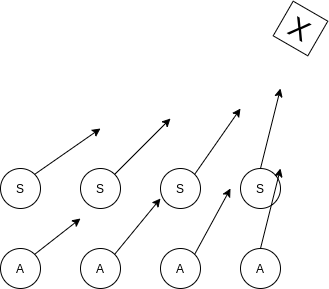
\includegraphics[width=0.35\textwidth]{imagenes/gdd/Following.png}
\caption{MockUp Seguimiento de la marca del jugador.}
\label{fig:mockup_following}
\end{figure}

En cuanto a las posibles formaciones para nuestras unidades, encontramos las siguientes:

\newpage

\begin{itemize}
\item \textbf{Sin formación:} las unidades no tendrán nigún paramétro de ordenación.

\begin{figure}[ht]
\centering
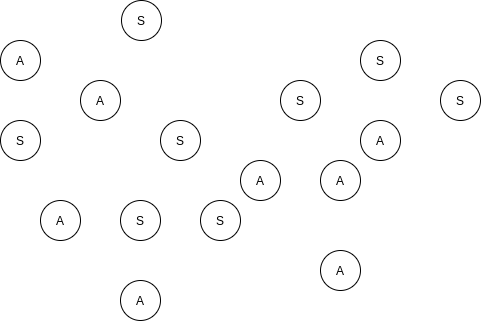
\includegraphics[width=0.32\textwidth]{imagenes/gdd/Formacion-desordenada.png}
\caption{MockUp unidades desordenada.}
\label{mockup_desordenada}
\end{figure}

\item \textbf{En anillo:} formación circular alrededor de una unidad especial. En caso de
no haber unidad escoltada el centro estará vacío. 
\end{itemize} 


\begin{figure}[ht]
\centering
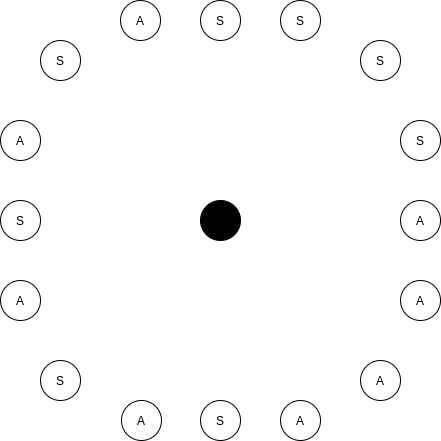
\includegraphics[width=0.32\textwidth]{imagenes/gdd/Formacion-anillo.png}
\caption{MockUp unidades en anillo.}
\label{mockup_anillo}
\end{figure}

Por último podemos ordenar a las unidades que mantengan una estrategia definida:

\begin{itemize}
\item \textbf{Huida:} en este modo las unidades seguirán el marcador sin pararse a pelear con unidades
cercanas enemigas.

\item \textbf{Agresivo:} en el momento en el que la tropa divisa un enemigo saldrá directo a atacarle,
aunque se aleje esta le seguirá mientras siga en su rango de detección.
\end{itemize} 

Aunque el jugador marque una estrategia y forma de plantear el combate, las unidades podrán
decidir si seguir al jugador o revelarse. Si los soldados cercanos están siendo masacrados
existe la posibilidad de que tengan miedo y huyan. Si las unidades enemigas nos superan en número
la unidad puede decidir si permanecer en defensa en lugar de atacar de forma activa.

\section{Unidades}
Entre las unidades podemos encontrar dos arquetipos con carácteristicas propias
que nos permitiran crear variedad en las soluciones a la hora de superar el
nivel.

Los tipos son los siguientes:
\begin{itemize}
	\item \textbf{Soldado:} es la unidad más básica que podemos encontrar en el campo de
							guerra, esta armado con una espada y posee estadísticas
							bajas.
	\item \textbf{Arquero:} va equipado con arco y flechas para atacar a distancia a
							sus rivales. Tiene menos resistencia que los soldados por
							lo que tendremos que protegerlos para asegurar su
							supervivencia.
\end{itemize}

\begin{table}[ht]
\begin{center}
\begin{tabular}{|c|c|c|c|c|}
\hline
        & Daño & Vida  & Rango  & Tiempo de ataque \\ 
\hline
\hline
Soldado & 7    & 24    & Melee & 2 seg.\\ 
\hline
Arquero & 4    & 14    & Largo & 3 seg.\\ 
\hline
\end{tabular}
\caption{Unidades y estadísticas}
\end{center}
\end{table}

\section{Controles}
A la hora de jugar tendremos una serie de teclas asignadas a las acciones que el
jugador puede realizar cuando interactúe con el juego. Para enumerarlas dividiremos las
acciones en dos grupos, dependiendo de si son para navegar por los menús o si
representan acciones durante el \textit{gameplay}.

Para avanzar por los menús usaremos la tecla \textbf{Enter} una vez estemos sobre la opción deseada o
para avanzar los mensajes explicativos del tutorial/informativos.

Las asignadas para jugar son las siguientes:
\begin{itemize}
	\item \textbf{Flechas o W/A/S/D:} mediante estas teclas podremos desplazar el puntero por el mapa.
	\item \textbf{Barra Espaciadora:} con esta otra podremos ordenar atacar a nuestras unidades,
									  si no encuentran una unidades enemiga en su rango se mantendrá
									  en seguimiento del puntero.
	\item \textbf{Ctrl:} activa el modo huída y las unidades dejarán de combatir y seguirán el
					  puntero.	
	\item \textbf{Z:} activa la formación en anillo.									  
	\item \textbf{X:} desactiva toda formación.
	\item \textbf{Ratón:} interactuar con el \textit{HUD}.
\end{itemize}

Tanto la \textbf{formación} como el \textbf{comportamiento} de las unidades se podrá cambiar desde un
pequeño \textbf{\textit{HUD}},que se encuentra en la esquina inferior izquierda.

\section{Pantallas}
Al ejecutar el programa la primera pantalla que aparecerá será la de 
inicio. Se compone del título del juego, la fecha de lanzamiento,
el nombre del desarrollador y un mensaje que nos indica que tenemos que pulsar la tecla
\textit{enter} para continuar, esta pantalla se mantendrá hasta que el jugador presione
dicha tecla.\\
Una vez pulsado el botón indicado se procederá a cargar el juego mientras se muestra
una barra que indica el progreso de cargado.

\begin{figure}[h]
\centering
\begin{minipage}[c]{0.42\linewidth}
	\hspace{9mm}
	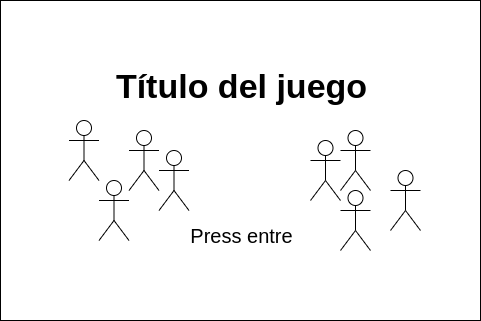
\includegraphics[width=0.7\textwidth]{imagenes/gdd/pantallas/Pantalla_ini.png}
	\caption{MockUp inicio.}
	\label{mockup_ini}
\end{minipage}
\begin{minipage}[c]{0.42\linewidth}
	\hspace{9mm}
	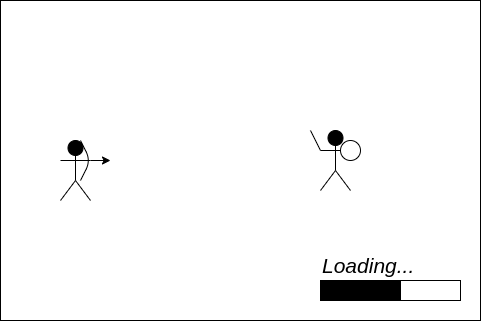
\includegraphics[width=0.7\textwidth]{imagenes/gdd/pantallas/Pantalla_carga.png}
	\caption{MockUp carga.}
	\label{mockup_carga}
\end{minipage}	
\end{figure}

A continuación de la carga nos encontraremos con el escenario, donde se desarrollará el
\textit{gameplay} y nos mantendremos en esta pantalla hasta que termine el juego, ya sea
por victoria o derrota del jugador.

\begin{figure}[ht]
\centering
\begin{minipage}[c]{0.45\linewidth}
	\hspace{9mm}
	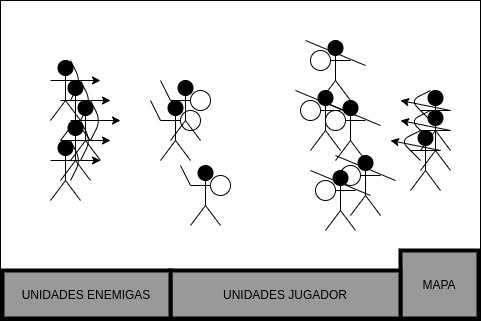
\includegraphics[width=0.7\textwidth]{imagenes/gdd/pantallas/Pantalla_gameplay.png}
	\caption{MockUp juego.}
	\label{mockup_juego}
\end{minipage}
\begin{minipage}[c]{0.45\linewidth}
	\hspace{9mm}
	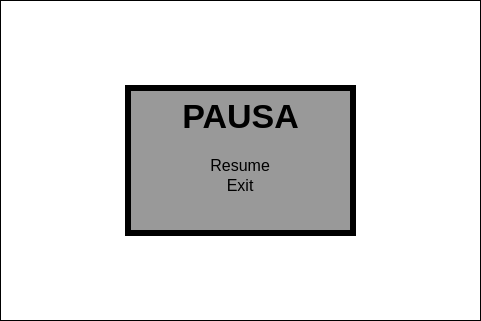
\includegraphics[width=0.7\textwidth]{imagenes/gdd/pantallas/Pantalla_pausa.png}
	\caption{MockUp pausa.}
	\label{mockup_pausa}
\end{minipage}	
\end{figure}

El final de la partida nos trae dos posibles escenarios, la victoria y la derrota. 
Para cada uno saldrá su respectivo mensaje y pasado un momento se nos mandará automáticamente a 
la pantalla de inicio.

Una última pantalla con la que el jugador podrá interactuar es la del menú de
pausa, en el cual se le dará la opción de salir o de volver a la
partida, mientras esta pantalla este activa la acción en el juego se paralizará hasta
que el jugador decida. 

\begin{figure}[ht]
\centering
\begin{minipage}[c]{0.45\linewidth}
	\hspace{9mm}
	
\includegraphics[width=0.7\textwidth]{imagenes/gdd/pantallas/Pantalla_victoria.png}
	\caption{MockUp victoria.}
	\label{mockup_victoria}
\end{minipage}
\begin{minipage}[c]{0.45\linewidth}
	\hspace{9mm}
	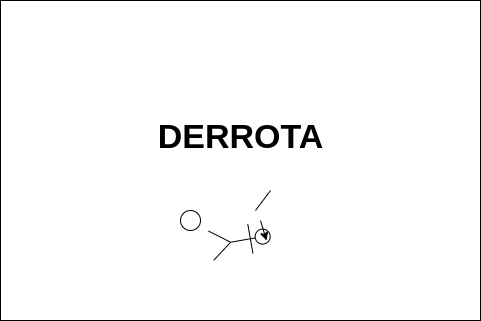
\includegraphics[width=0.7\textwidth]{imagenes/gdd/pantallas/Pantalla_derrota.png}
	\caption{MockUp derrota.}
	\label{mockup_derrota}
\end{minipage}	
\end{figure}

\section{Estados del juego}
Una vez mostradas todas las posibles pantallas con las que podrá interactuar el jugador,
es interesante dibujar un diagrama de flujo que plasme sus conexiones y posibilidades
con el fin de crear una representación gráfica que sirva como esquema global.

Dicho esquema podemos encontrarlo en la figura siguiente:

\begin{figure}[ht]
\centering
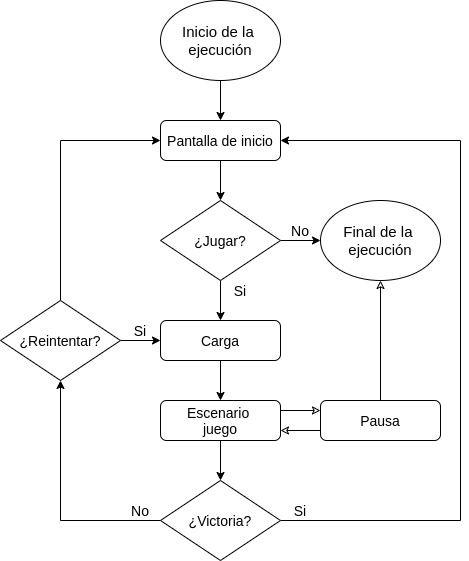
\includegraphics[width=0.45\textwidth]{imagenes/gdd/pantallas/flow_ejecucion.png}
\caption{MockUp flujo de ejecución.}
\label{esq:flow_juego}
\end{figure}

\section{Niveles}
El juego contiene actualmente 2 niveles, el primero se trata de un nivel introductorio
en el que encontraremos grupos pequeños de unidades fáciles de abatir para que el jugador conozca
cómo es el combate en el juego. Además, a lo largo del nivel pondrémos marcadores para que indiquen
al jugador cómo jugar o \textit{tips} para superar los niveles de forma satisfactoria.
El nivel se supera matando a los enemigos.

\begin{figure}[ht]
\centering
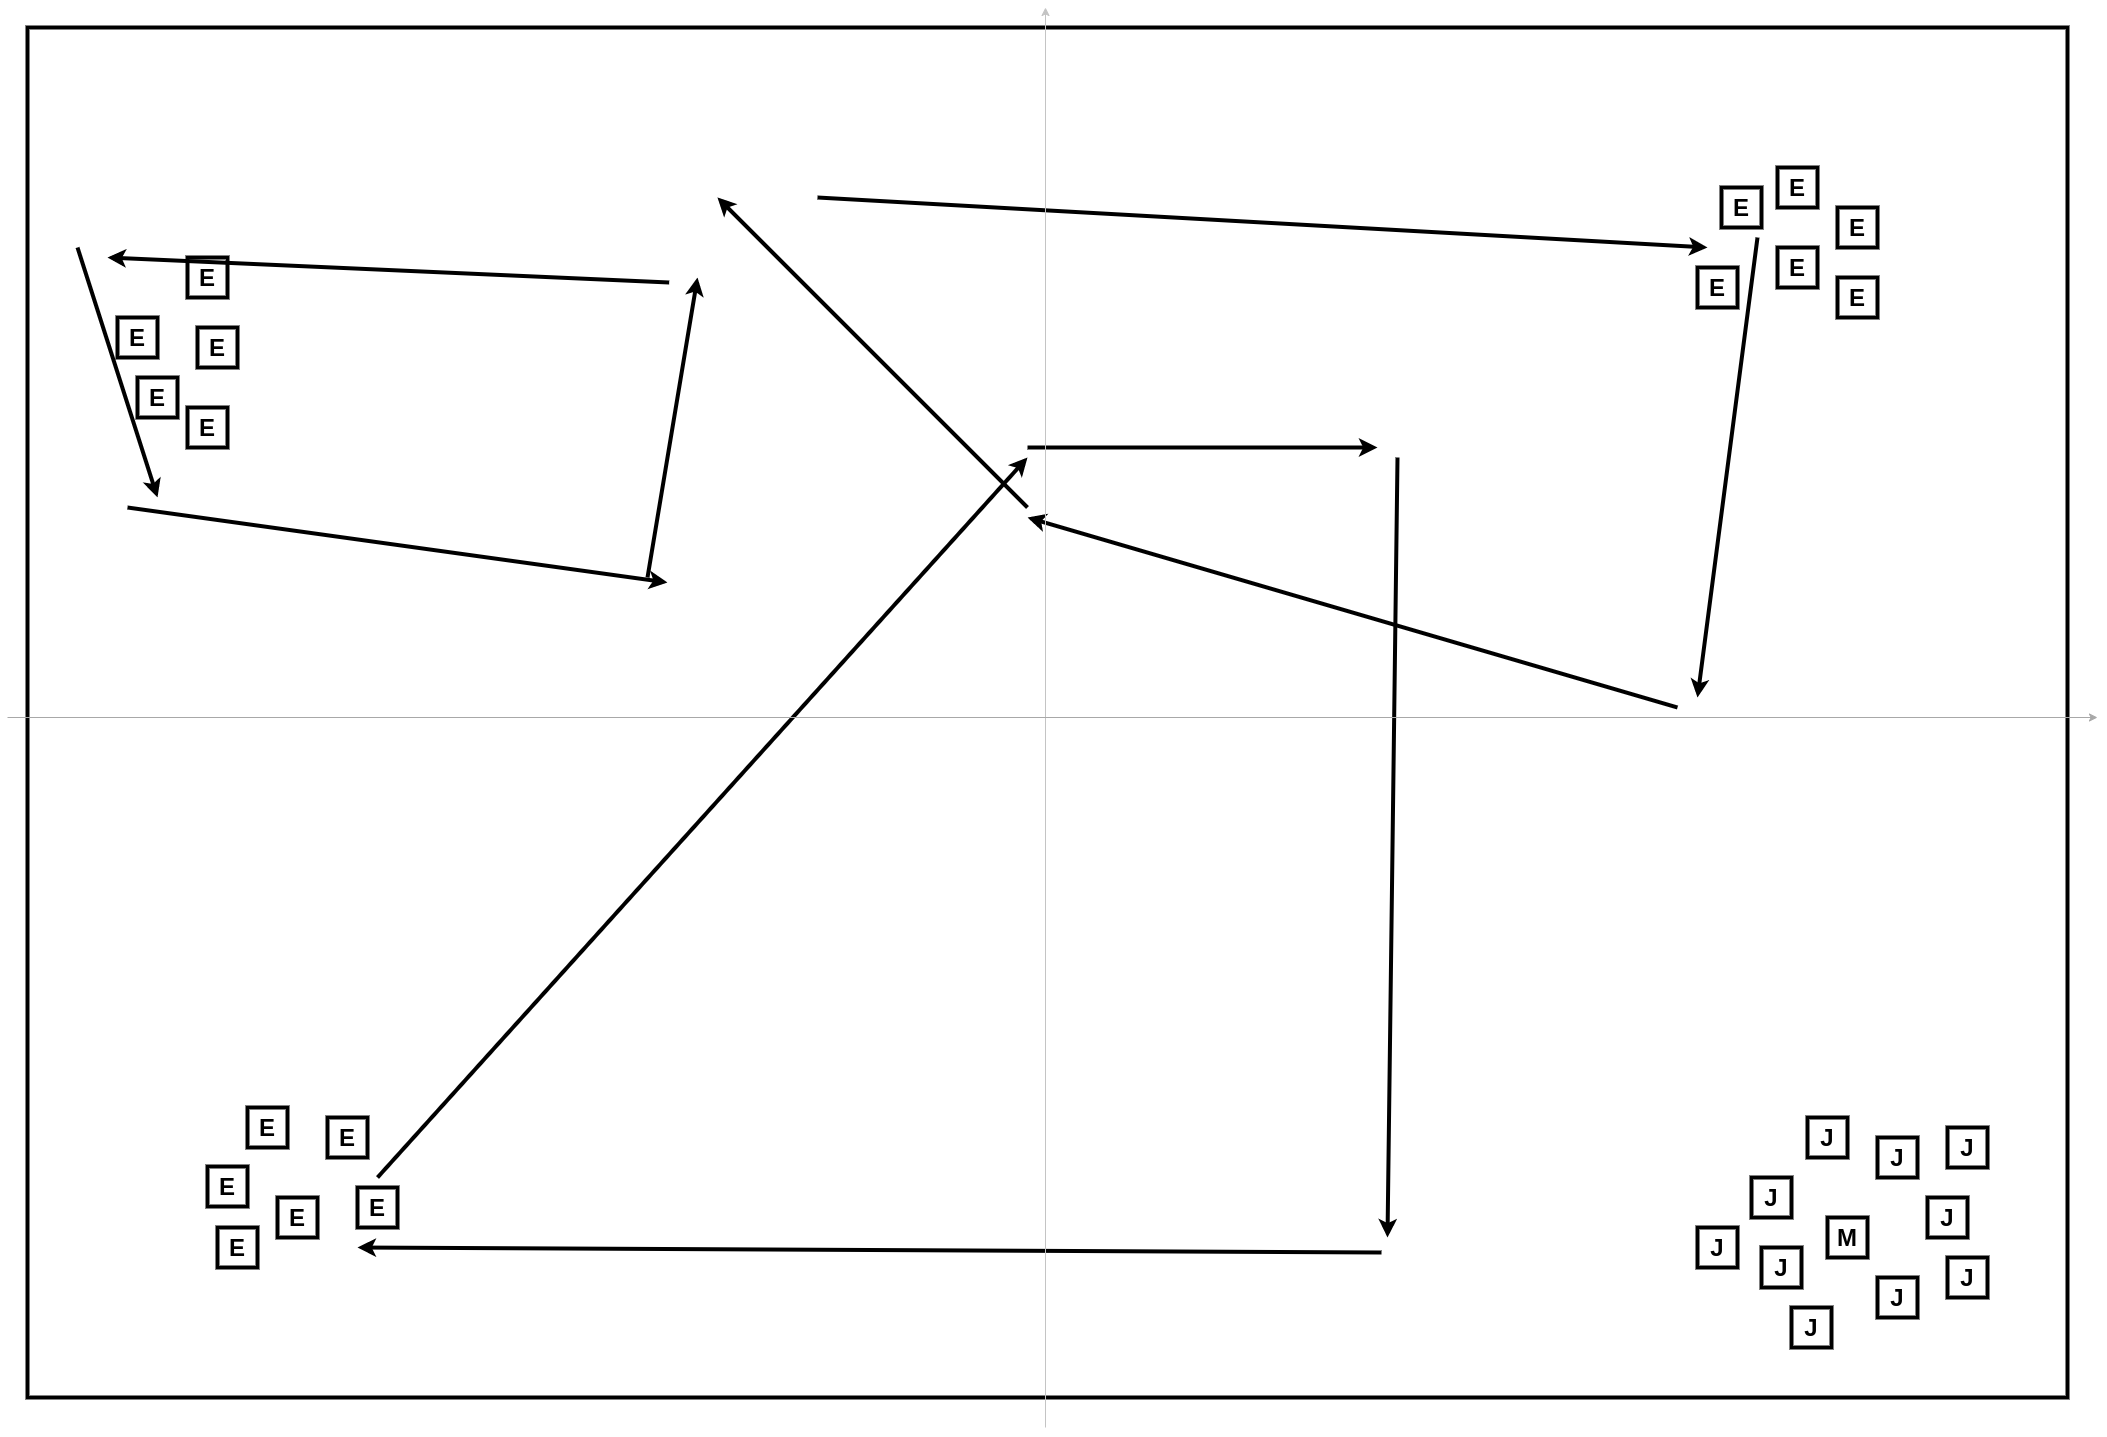
\includegraphics[width=0.6\textwidth]{imagenes/gdd/nivel0.png}
\caption{MockUp nivel 0.}
\label{esq:lvl0}
\end{figure}

En el segundo nivel se muestra otro de los objetivos posibles en el juego: alcanzar
una zona de huída/meta más allá de las tropas enemigas. En este nivel encontraremos
grupos más grandes de enemigos que nos pueden vencer y hacernos repetir el nivel, por ello podremos optar
por intentar derrotarlos o buscar una ruta que nos evite el conflicto lo máximo posible. 

\begin{figure}[ht]
\centering
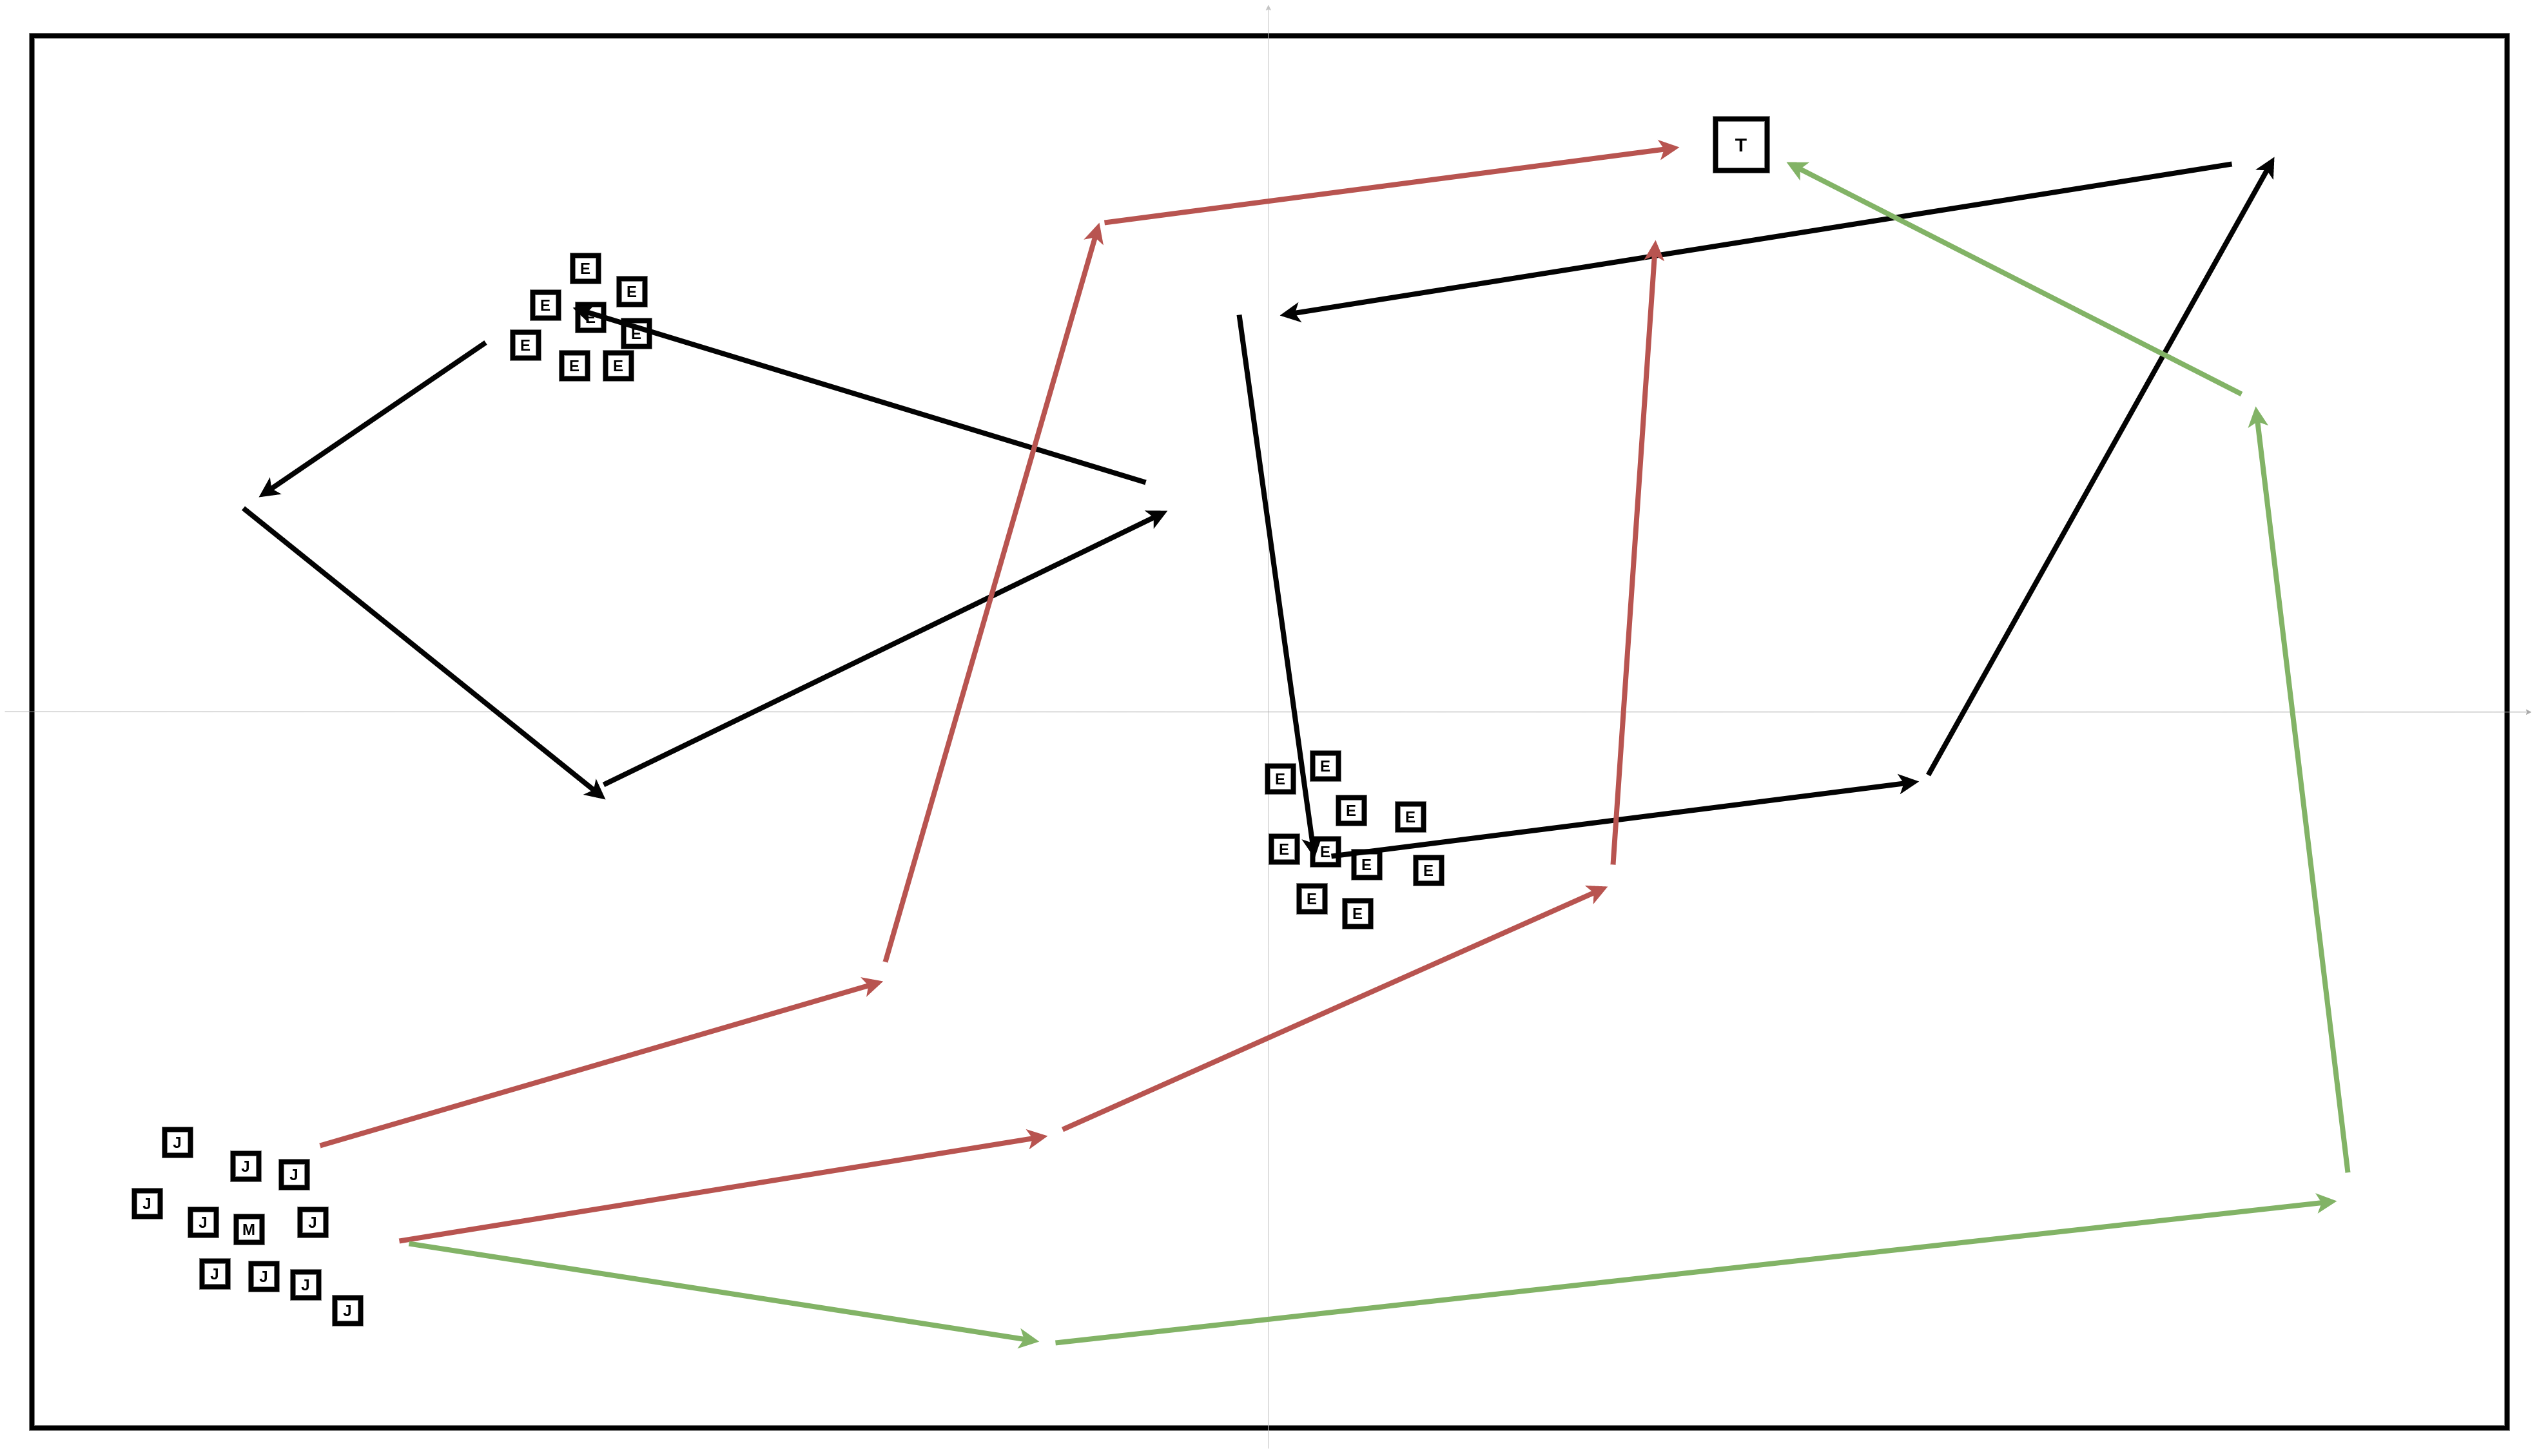
\includegraphics[width=0.6\textwidth]{imagenes/gdd/nivel1.png}
\caption{MockUp nivel 1.}
\label{esq:lvl1}
\end{figure}

\section{Escenarios}
A lo largo de los niveles la intención es que nos encontremos con distintos biomas como
pueden ser praderas, bosque o desiertos similares a los que podemos encontrar en \ac{AoE} II.

\begin{figure}[ht]
\centering
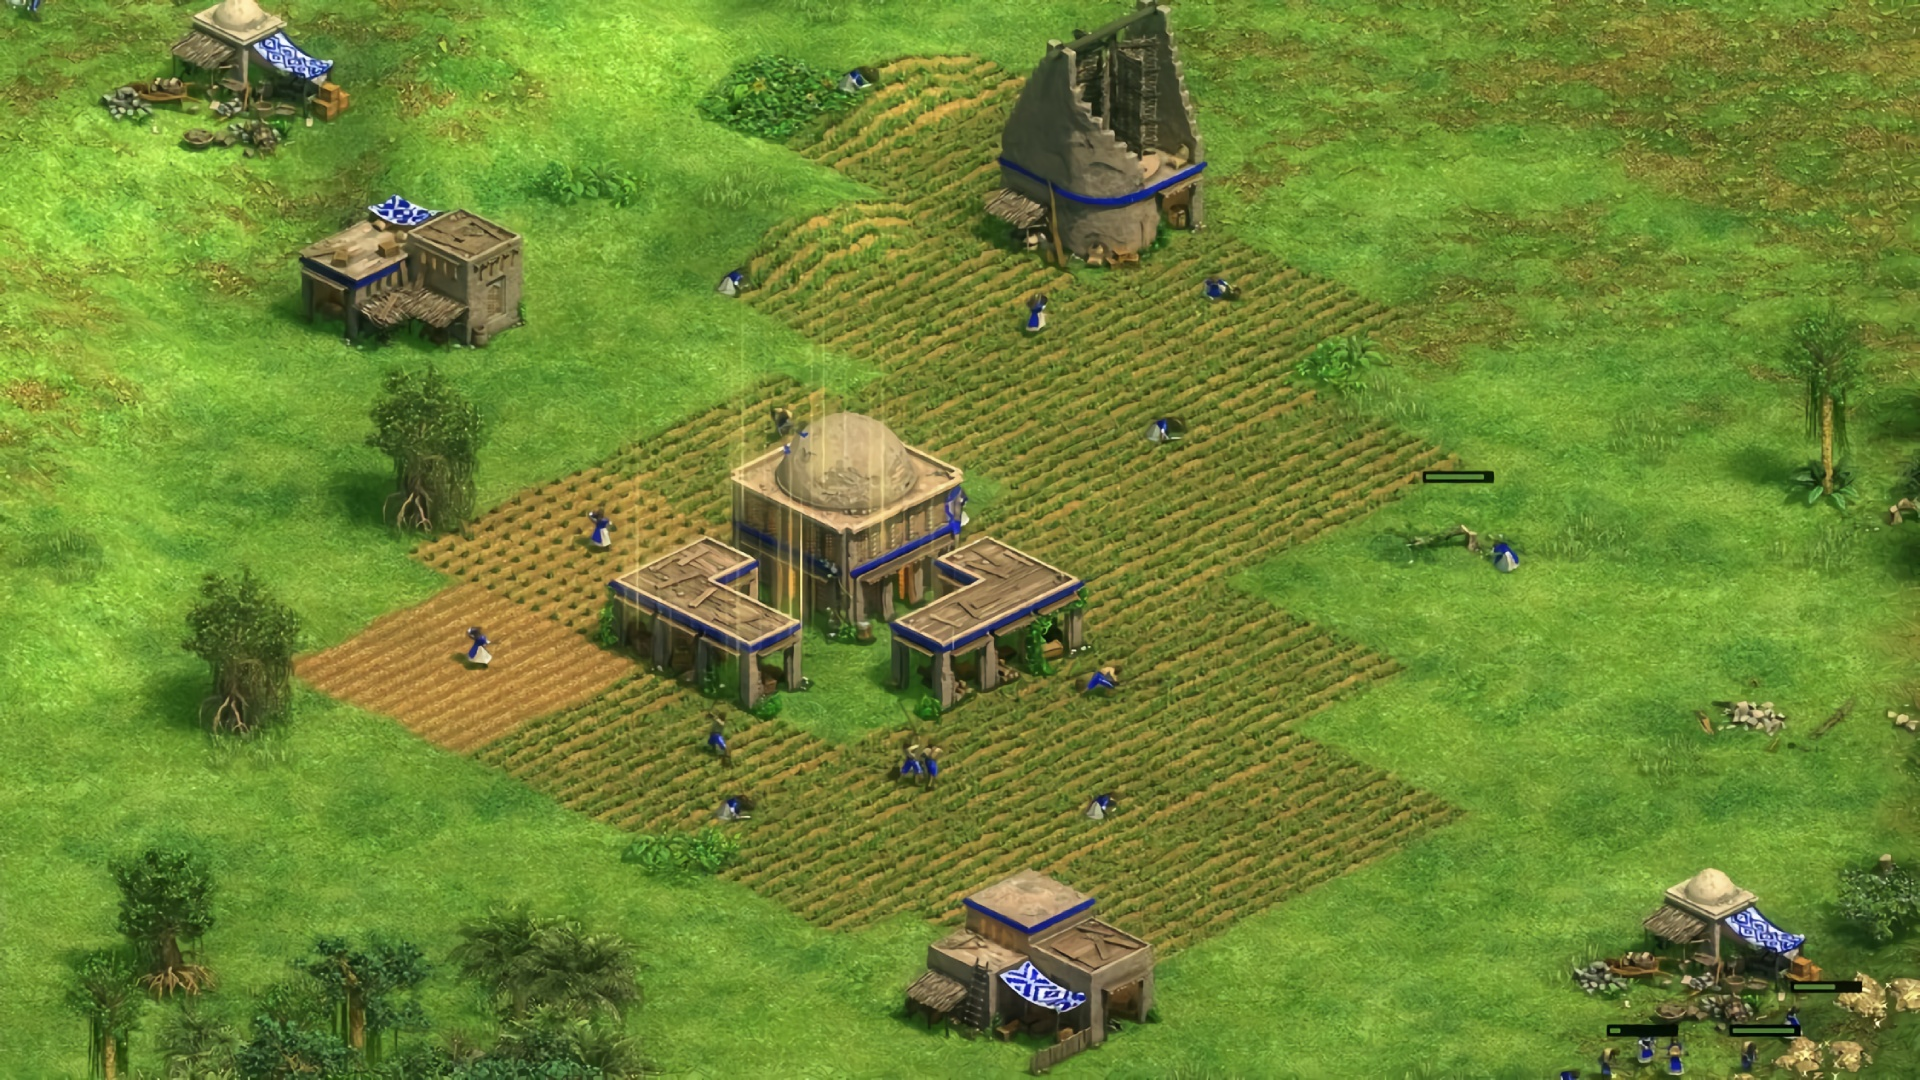
\includegraphics[width=0.6\textwidth]{imagenes/gdd/mapa_aoe_1.jpg}
\caption{Ejemplo escenario con vegetación.}
\label{img:mapa_aoe1}
\end{figure}

Además de imitar el estilo artístico el juego se desarrollará empleando una cámara
aerea fija manteniendo una perspectiva isométrica que nos permitirá visualizar desde
un punto elevado una gran porción del escenario. Esto lo haremos con el fin de dar al
jugador la posibilidad de conocer lo máximo posible el territorio cercano y a la
vez le libramos de preocuparse por situar la cámara para cada momento. \\
Al mantener una posición fija podemos situar todos los elementos en la escena de forma
que no obstaculicen la visión o molesten al jugador.

En las primeras versiones del proyecto el juego todos los elementos serán 2D y la vista será
un plano picado, el final deseable será poder pasar a un entorno 3D.

\section{Sistema de cámaras}
Si quisiéramos mostrar todo el nivel por pantalla, tendríamos el problema de que los elementos
quedarían dibujados con un tamaño demasiado pequeño si el nivel supera las dimensiones de la pantalla.
Por ello, si queremos poder diseñar niveles con las dimensiones que queramos deberemos mostrar únicamente
las fracción del nivel que ocupamos en cada momento.

En este caso, tendríamos una cámara que seguirá al puntero del jugador por el nivel y tendremos el
minimapa para poder ubicarnos en el nivel.

\section{Mínimo producto viable}
Una vez planteadas todas las características deseadas para el videojuego, es acosenjable
decidir qué partes del producto son vitales para mostrar la experiencia
de juego deseable. El hecho de marcar estos objetivos nos ayudará a poder desarrollar una
versión reducida del proyecto que nos permita dar la sensación de tener un producto acabado.\\
Es importante realizar este proceso ya que por motivos internos o externos al equipo de desarrollo,
siempre existen contratiempos que nos impidan conseguir todos los objetivos propuestos en el
documento.

En cuanto a las etapas en la ejecución del juego, encontramos esencial el poder finalizar el nivel,
ya sea por victoria o derrota. Acto seguido volver al comienzo del nivel, dejando a un lado un
posible menú inicial y de pausa.

Una vez en partida el juego constará de un nivel único compuesto por: un escenario estático
mínimo, un conjunto de unidades propiedad del jugador y otro perteneciente a la máquina.\\
Al inicio del juego el jugador se encontrará quieto en uno de los extremos del nivel y el enemigo 
estará patrullando por una zona designada, dejando así a elección del jugador la distribución y el
momento exacto en el que comenzará la disputa.

En lo referente a las mecánicas y jugabilidad, es importante que el jugador sea capaz de poder
mover a sus unidades por el escenario y ordenarles atacar. También sería deseable poder
ajustar algunos parámetros del comportamiento de su ejercito para poder pasar el nivel de más
de una forma.\\
Por otro lado, la \ac{IA} debe ser capaz de detectar el acercamiento del jugador y responder a la
ofensiva, dejando la capacidad de tomar la iniciativa y variar su estrategia para versiones
más completas. Ambos ejércitos se compondrán de soldados y arqueros.

En lo referente al apartado visual, sería deseable tener sprites para unidades y escenario pero
de ser necesario podemos mantener el sistema de \textit{render} inicial.


\section{Actualización: 13/04/21}
\begin{itemize}
	\item Corregido el movimiento lento de las entidades en algunos momentos cuando estaban en el radio
	de frenada debido a un cálculo erróneo en las diviones con el tipo de dato en coma fija.
	
	\item Creación de una componente para las colisiones e integración en los sistemas pertinentes.
	
	\item Solucionado el problema de las balas que no colisionaban bien.
	
	\item Adicción de los \textit{Colliders} al modo de depuración visual.
	
	\item Cambios ligeros en el sistema de eventos de las balas y creación y destrucción de entidades.
	
	\item Creación de un \textit{HUD} para seleccionar comportamientos y formaciones de las unidades
	aliadas.
	
	\item Rediseño completo en la toma de decisión de las unidades aliadas y enemigas.

	\item Creación de un componente de BlackBoard para el seguimiento al pj v0.1.
	
	\item Sistema de cámaras y coordenadas de mundo: ahora las dimensiones del nivel son independientes
	del tamaño de la ventana, se usan los limites del nivel para no dejar pasar a las unidades, se hace
	\textit{clipping} sobre las unidades que no están en la cámara, el minimapa ahora muestra la porción
	de nivel que se muestra.
	
	\item Se ha mejorado el sistema de entidades objetivo y los mensajes de muerte y ataque para cambiar
	de objetivo cuando el actual muera, además al morir una unidad se eliminan los demás mensajes asociados
	a ella.

	\item El componente de \ac{IA} ya no contiene la ruta directamente, ahora contiene un iterador a su
	ruta y se ha creado el tipo de dato ruta con operadores sobrecargados para navegar por ella. También
	tenemos ``caminos'' diseñados pero sin incluir, los cuales son caminos no cíclicos.

	\item Se ha ampliado un poco el GDD con apartados sobre tareas pendientes y objetivos.

	\item En el diario de desarrollo se han sustituido códigos de ejemplo por mockups.  
\end{itemize}

\section{Actualización: 06/05/21}
\begin{itemize}
	\item Redacción problema en las divisiones de los enteros con coma fija.

	\item Redacción problema con las colisiones y solución.

	\item Redacción \textit{HUD} v0.4.
	
	\item Redacción sistema de cámaras en el GDD y diario de desarrollo.

	\item Redacción cambios en las entidades: rutas y comportamientos.
\end{itemize}

\chapter{Metodología y fases del producto}
\label{metodologia}
\section{Metodología}
La metodología llevada a cabo durante el proyecto es una creación propia basada en caraterísticas
copiadas de metodologías ágiles como el \textbf{'Scrum'} y adaptadas a la forma de trabajar propia.
La idea es estructurar todo el proyecto en diversas iteraciones y durante estas marcarse
objetivos y/o tareas con el fin de añadir funcionalidades completas.

El uso de \textbf{iteraciones} para dividir la carga de trabajo y agrupar tareas nos ayudará
a conseguir acotar la duración de algunas tareas y marcarnos objetivos a corto/medio
plazo. Además de separar por funciones el proyecto, las tareas que conllevan su desarrollo
también deberemos analizarlas e intentar reducir su tamaño y carga lo máximo posible, esto
permite obtener una sensación de éxito de forma rápida lo cual ayuda a mantener una moral y 
motivación altas.

Para poner un ejemplo de como elaborar esta separación por subtareas, el objetivo que vamos a
usar es ``dibujar elementos por pantalla''. Como estamos en un proyecto básado en \ac{ECS} rápidamente
vemos que vamos a requerir mínimo un componente de dibujado \textit{(RenderCmp)} y un 
``RenderSystem'' el cual se encargará de recoger todos los elementos visuales y hacer las
llamadas necesarias para dibujarlos. \\
En caso de no tener una librería de dibujado, otra tarea podría ser el buscar una que sea capaz
de realizar el trabajo requerio y/o implementar una propia
\footnote{Esto supondría una serie de tareas en base a la cantidad de funcionalidades que se requieran.}. 

Para ayudar a la planificación del trabajo usaremos la herramienta `Trello'
~\ref{fig:logos} \footnote{Página de `Trello': https://trello.com/es}
la cual nos permitirá crear diversas listas según el ámbito o el estado de
desarrollo de las distintas tareas que contendrán, cada tarea se ve representada con
una tarjeta la cual puede tener una serie de subtareas asociadas dentro. Esto nos
permitirá tener un registro de todas las labores que quedan por hacer en cada iteración y
cuales ya estan termiandas completamente, además podremos conservar las listas de las tareas
realizadas en iteraciones anteriores para futuras revisiones.

Otra herramienta de control que usaremos durante el desarrollo será `Toggl'
~\ref{fig:logos} \footnote{Página de `Toggl': https://toggl.com}
la cual nos permitirá llevar a cabo un registro de las horas que dedicamos en cada tarea
y agrupar tareas en función del campo de estudio o parte del desarrollor al que pertecen.

\begin{figure}[ht]
\centering
\begin{minipage}[c]{0.45\linewidth}
	\hspace{1cm}
	
\includegraphics[width=0.7\textwidth]{imagenes/metodologia/logo-trello.png}
\end{minipage}
\begin{minipage}[c]{0.45\linewidth}
	
\includegraphics[width=0.7\textwidth]{imagenes/metodologia/logo-toggl.png}
\end{minipage}	
\caption{Logos de Trello y Toggl.}
\label{fig:logos}
\end{figure}

\section{Iteraciones}
En esta sección se comentarán brevemente los objetivos planteados y las tareas que
se han llevado a cabo en cada iteración adjuntando el tablero de `Trello' asociado.

\subsection{Iteración 0}
Esta iteración tenía como proposito terminar de definir la idea para el
proyecto, ya que, todavía era un poco difusa la imagen del producto final que se quería desarrollar.
Para ir entrando en una dinámica productiva e ir definiendo lo que se quería hacer,
comenzamos por iniciar el desarrollo de un propotipo a la vez que preparabamos un poco
los materiales relacionados con la memoria, como puede ser la lectura de las directrices
y/o la revisión de la plantilla de \LaTeX~\ref{img:it_0}.

Al final de esta iteración el prototipo contaba con una versión básica del bucle principal
del juego donde creamos una serie de sistemas, \textit{managers} y entidades además del dibujado
y movimiento\footnote{En esta versión nos limitamos a un ``Goto'' a través de 4 puntos.} de 
estas.

\begin{figure}[ht]
\centering
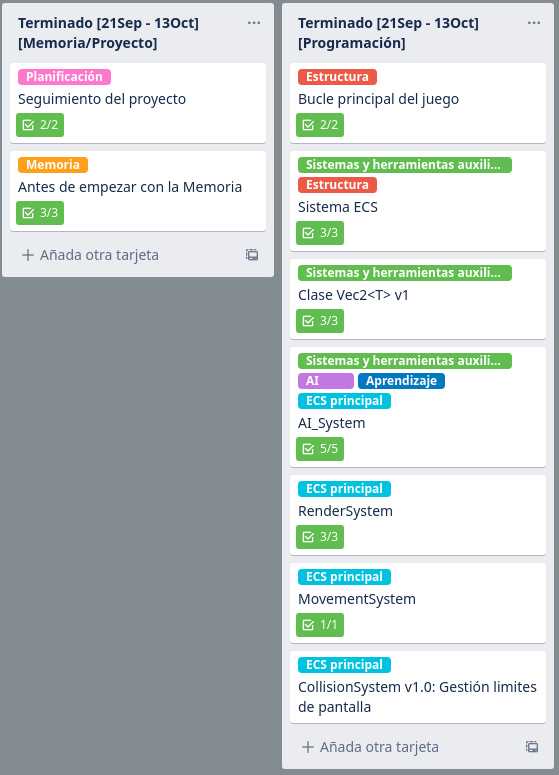
\includegraphics[width=0.45\textwidth]{imagenes/metodologia/tareas_it0.png}
\caption{Lista de tareas realizadas en la iteración 0}
\label{img:it_0}
\end{figure}

\subsection{Iteración 1}
A lo largo de esta iteración seguimos añadiendo sistemas al prototipo como puede ser el
de \textit{Input} el cual nos permitirá interactuar con el producto, además de herramietas
como el mapeado del teclado o el tipo de dato en coma fija en el cual profundizaremos más tarde.

Por otro lado, se comenzó a trabajar en la \ac{IA} del juego creando los primeros comportamientos
y herramientas para cambiar entre ello. Como veremos más adelante también, aquí caeremos en los primeros
errores de concepto a la hora de trabajar con los \textit{`Steering behaviors'}.

Por último, finalizamos la introducción en el uso de \LaTeX, \textit{`JabRef'} y la plantilla comenzando 
así con la redacción de esta memoria~\ref{img:it_1}.

\begin{figure}[ht]
\centering
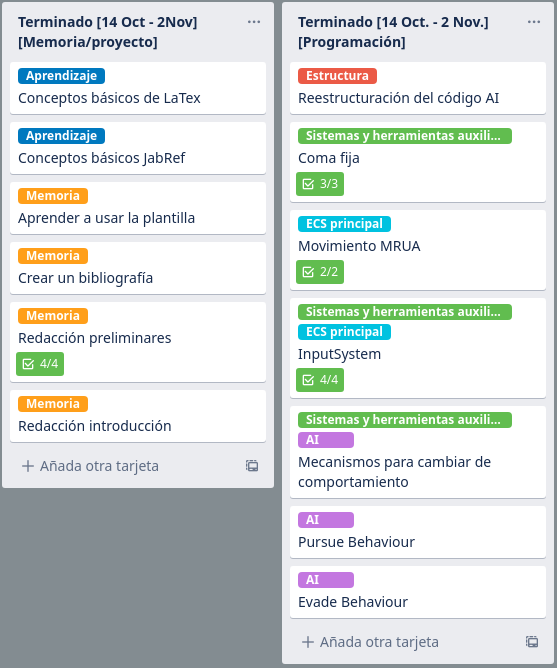
\includegraphics[width=0.45\textwidth]{imagenes/metodologia/tareas_it1.png}
\caption{Lista de tareas realizadas en la iteración 1}
\label{img:it_1}
\end{figure}

\subsection{Iteración 2}
Durante esta tercera iteración los objetivos eran los de corregir el funcionamiento de los
\textit{`Steering behaviors'}, añadir elementos visuales que ayuden al debug de la \ac{IA}
mostrando las componentes del movimiento de las entidades y herramientas para el control del
tiempo de ejecución y el tamaño del \textit{`DeltaTime'}.

Como podemos apreciar en la lista~\ref{img:it_2}, las tareas de control de la ejecución del
programa no fueron realizadas a tiempo, en su lugar se le dió prioridad a mejorar el uso
de la coma fija para un código más limpio y crear metodos auxiliares como puede ser el paso de
coordenadas continuas a pixeles en pantalla, permitiendo así trabajar a lo largo del programa 
usando enteros con signo y procesarlos en el sistema de \textit{`Render'}.

En lo referente a la memoria comenzamos la redacción de una versión preliminar del \ac{GDD},
Estado del Arte y metodología. 

\begin{figure}[ht]
\centering
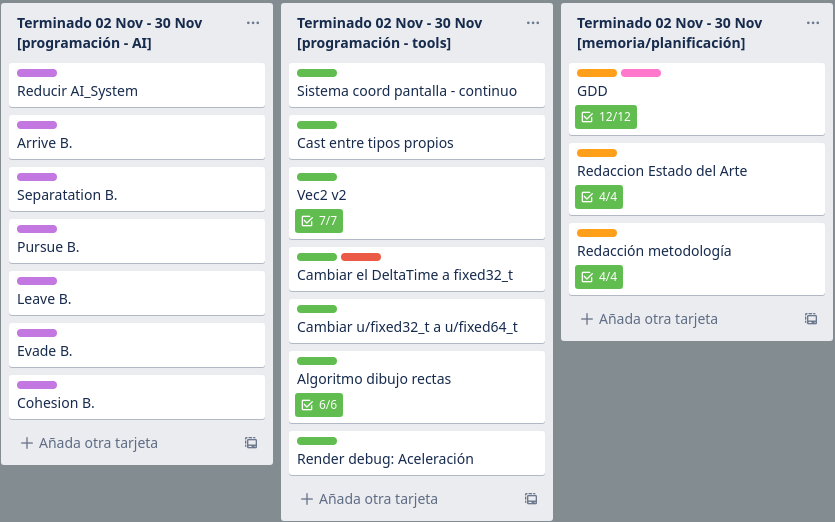
\includegraphics[width=0.65\textwidth]{imagenes/metodologia/tareas_it2.png}
\caption{Lista de tareas realizadas en la iteración 2}
\label{img:it_2}
\end{figure}


\chapter{Desarrollo y fases del producto}
A lo largo de esta sección comentaremos todo el proceso de desarrollo del prototipo y de la 
memoria, las diferentes iteraciones del producto serán agrupadas en diversas fases con el fin
de facilitar la lectura y el entendimiento de los objetivos planteados en cada momento. Además,
se contarán de forma más extensa los puntos relevantes y objetivos en este proyecto.

\begin{longtable}[c]{|c|c|c|}
\hline
Terminado es esta iteración & Terminado en otra iteración & Sin definir cuando se terminará \\ 
\hline
			(vacio)			&             It.X            &             $\infty$            \\ 
\hline
\caption{Leyenda finalización de tareas.}
\end{longtable}

\section{Fase 0: Definición del proyecto y primeros pasos}
\begin{longtable}[c]{|p{7cm}|c|c|}
\hline
Iteraciones                                               & \% Completado    & Terminado en \\
\hline
\endhead
\textbf{0.1.} Definir la idea.                              & 60\%          & It.2         \\
	\cmidrule[.006pt]{1-3}
\textbf{0.2.} Iniciar desarrollo del prototipo
				Integrar TinyPTC y dibujar por pantalla.    & 100\%         &              \\
	\cmidrule[.006pt]{1-3}
\textbf{0.3.} Adquirir hábito de escribir, preparar
				las herramientas y entorno de LaTex.        & 50\%          & It.2         \\
	\cmidrule[.006pt]{1-3}
\textbf{0.4.} Prototipado del movimiento usando 
				\textit{Steering behavior}.                 & 30\%          & It.1         \\

\cmidrule[1pt]{1-3}

\textbf{1.1.} Creación tipo con coma fija.                  & 100\%         &         \\
	\cmidrule[.006pt]{1-3}
\textbf{1.2.} Busqueda de referentes.                       & 40\%          & It.3    \\
	\cmidrule[.006pt]{1-3}
\textbf{1.3.} Corregir funcionamiento de los
				\textit{Steering behavior} y
				prototipar todos los posibles.              & 100\%         &          \\
	\cmidrule[.006pt]{1-3}
\textbf{1.4.} Sistema de debug visual: vectores.            & 100\%         &          \\ 
	\cmidrule[.006pt]{1-3}
\textbf{1.5.} Herramientras control de ejecución.           & 50\%          & It.7     \\ 

\cmidrule[1pt]{1-3}

\textbf{2.1.} Trabajar más la memoria.                      & 65\%          & $\infty$ \\
	\cmidrule[.006pt]{1-3}
\textbf{2.2.} Terminar de definir idea (GDD).               & 100\%         &          \\
	\cmidrule[.006pt]{1-3}
\textbf{2.3.} Implementar el mínimo producto.               & 20\%          & It.4     \\
	\cmidrule[.006pt]{1-3}
\textbf{2.4.} Experimentación y análisis de resultados.     & 0\%           & It.8     \\
\hline
\caption{Resumen fase 0}
\end{longtable}

Esta primera fase engloba las tres primeras iteraciones donde comenzamos a terminar de definir 
la idea para el proyecto, ya que, todavía era un poco difusa la imagen del producto final que se
quería desarrollar.

\subsection*{Iteración 0: Bucle del juego y primeros sistemas}
Para ir entrando en una dinámica productiva iniciamos el desarrollo de funcionalidades básicas 
como pueden ser el bucle principal del juego, en el cual usamos de la librería \textit{\textless
chrono\textgreater} de C++ para medir y limitar el tiempo entre ejecuciones del bucle acompañado del uso 
de una enumeración que contiene los posibles resultados de un ciclo del juego.

\begin{figure}[htb]
\centering
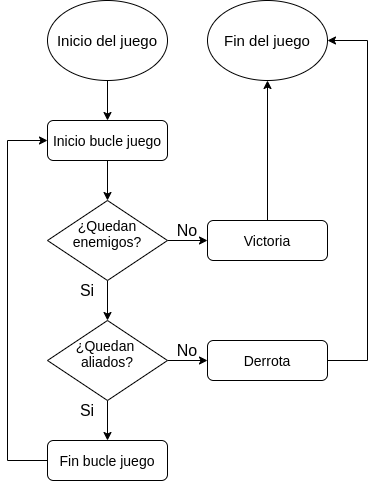
\includegraphics[width=0.4\textwidth]{imagenes/diario_desarrollo/Loop_juego.png}
\caption{Posibles resultados del bucle de juego.}
\label{fig:game_loop}
\end{figure} 

Una vez tenemos el bucle, toca introducir algo que hacer en el, como primer sistema del juego
encontramos el sistema de dibujado el cual se encargará de crear y manejar la ventana, además
de pintar nuestras entidades y herramientas visuales. Para incluir todas estas funcionalidades
sin añadir librerías pesadas incluiremos \textit{\textless TinyPTC\textgreater} de \newline
\citeauthor*{tinyptc2019}, la cual no 
incluye demasidas funcionalidades u opciones pero nos permitirá trabajar rápido y de forma 
sencilla. Los sprites en un inicio serán simples cuadrados de colores por lo que no requeriremos 
mucho.

Por último, se añadireron las componentes de movimiento e \ac{IA} que, junto a sus correspondientes
sistemas, nos permitirán poder crear un comportamiento de patrulla básico entre puntos fijos.
Además, se terminó la preparación de las herramientas de \LaTeX y `Jabref' para redactar la 
memoria acompañado de la lectura de las directrices, normas y memorias de compañeros del año 
pasado.

\subsection*{Iteración 1: Entero con coma fija e inicio de la IA}
A lo largo de la iteración siguiente, seguimos añadiendo funcionalidades al prototipo como puede 
ser el componente y sistema de \textit{Input}, el cual nos permitirá interactuar con el juego
mediante el mapeado del teclado haciendo uso de la librería \textit{\textless X11\textgreater}
y \textit{\textless TinyPTC\textgreater}.

Una de las herramientas implementadas en el proyecto es el tipo de dato entero con coma fija,
en C++ podemos encontrar el tipo fundamental \textit{float} creado para trabajar con números 
reales, pero si miramos como funcionan exactamente es posible encontar que no es lo que deseamos
exactamente. Los \textit{floats} usan ``precisión simple'' lo cual implica que conforme el número 
sea más grande, la cantidad de bytes destinados a la representación de la parte decimal va 
disminuyendo ofreciendo así menor precisión. Además, trabajar con ellos es más costoso a nivel
computacional\footnote{Esto pasa sobretodo en máquinas que no tengan CPUs con unidades destinadas 
a cálculos en coma flotante} y conllevan un código más pesado debido a la codificación usada 
al ser compilados.

El tipo con coma fija tiene dos partes, en primer lúgar el valor que se quiere reprentar normal
y corriente, y por otro la escala, número que indicará la cantidad de valores disponibles
para la representación decimal. La escala la usaremos para multiplicar o dividir nuestro número
para convertirlo a coma fija, devolverlo sin escalar y/o operaciones con otros números enteros.\\
Es importante elegir una escala adecuada para trabajar de forma eficiente, para ello escogeremos
un número portencia de 2 el cual nos permitirá usar desplazamientos en múltiplicaciones y divisiones,
hacíendo los calculos mucho más rápidos que si tuvieramos que usar las operaciones comunes.

\begin{figure}[htb]
\centering
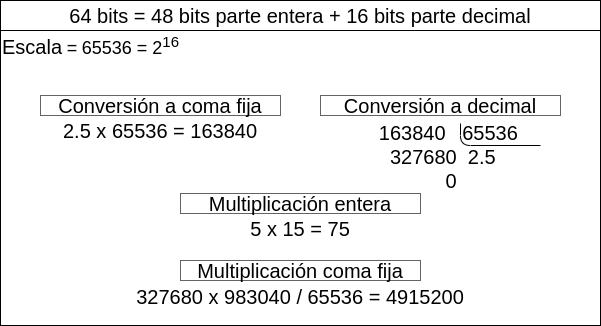
\includegraphics[width=0.8\textwidth]{imagenes/diario_desarrollo/Entero_fijo.png}
\caption{Ejemplos entero con coma fija.}
\label{fig:fixed}
\end{figure} 

Por otro lado, se comenzó a trabajar en la \ac{IA} del juego creando los primeros comportamientos
y herramientas para alternar entre ellos. Aquí caeremos en los primeros errores de concepto a la
hora de trabajar con los \textit{`Steering behaviors'}, ya que, a la hora de implementar los
usamos un plateamiento y cálculos de movimiento cinético sin aceleración, trabajando directamente 
con la velocidad.\\
En su lugar, lo planteado por la técnica es usar la aceleración de la entidad, de esta forma se 
logrará calcular el movimiento deseado en un momento puntual, enfrentándo lo contra la velocidad 
acumulada. Esto nos proporcionará un movimiento continuado y dinámico en lugar de cambiar drásticamente de 
dirección y velocidad.

\begin{figure}[htb]
\centering
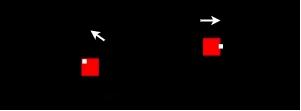
\includegraphics[width=0.35\textwidth]{imagenes/diario_desarrollo/mov1.png}
\caption{Movimiento rectilíneo uniforme.}
\label{fig:mru}
\end{figure} 

\begin{figure}[htb]
\centering
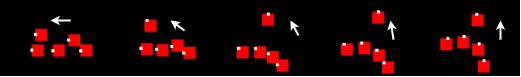
\includegraphics[width=1\textwidth]{imagenes/diario_desarrollo/mov2.png}
\caption{Movimiento rectilíneo acelerado.}
\label{fig:mra}
\end{figure} 

Uno de los comportamientos más sencillos es el \textit{`Arrive'}, el cual nos
llevará a la posición objetivo de forma directa y conforme estemos llegando a esta, la 
acceleración disminuirá parando una vez hayamos llegado al destino. En esta función podremos
apreciar como calculamos la velocidad objetivo en función de la distancia hasta llegar a
la posición objetivo, una vez se calcula se compara con el desplazamiento actual de la entidad
y es la resta de ambas la que nos dará la acceleración necesaria para alcanzar la velocidad
objetivo, siempre controlando que la acceleración y la velocidad no exceden los límites 
marcados.\\
Además, contamos con dos modeficadores adicionales como son el tiempo deseado para alcanzar el
objetivo y un límite de distancia con el objetivo para evitar solapes y/o oscilar sobre el.

\begin{figure}[htb]
\centering
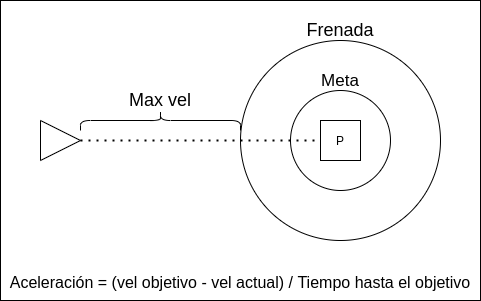
\includegraphics[width=0.75\textwidth]{imagenes/diario_desarrollo/arrive_b.png}
\caption{Diagrama Arrive Behaviour.}
\label{fig:arrive_b}
\end{figure} 

\subsection*{Iteración 2: Herramientas de depuración visual y tiempo de ejecución}
Durante la tercera iteración nos centramos en la mejora de algunos \textit{`Steering behaviors'}
para terminar de hacerlos más fáciles de usar y combinar, con el fin de tener un código más 
limpio y legible, también se mejoró el uso de la coma fija añadiendo más operaciones y ajustando
el funcionamiento.

En cuanto al \textit{'Flocking'}, se comenzó a trabajar en el calculo de las distintas fuerzas que
actuarán sobre las unidades, siendo estas: la atracción al centro de masas del grupo y la separación
de las unidades cercanas. En ambos casos, se recorre el array de entidades aliadas seleccionando las
que se encuentren dentro del radio de influencia, el módulo del vector dependerá de la distancia entre
ambas entidades siendo las más cercanas la que tengan más presencia en la separación y las más lejanas 
en la cohesión, una vez se terminan de acumular todas las direcciones se comprueba que la fuerza 
resultante no es superior al límite.

\begin{figure}[ht]
\centering
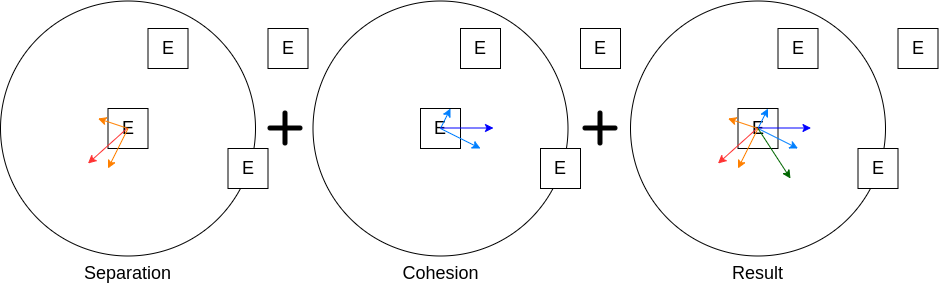
\includegraphics[width=0.95\textwidth]{imagenes/diario_desarrollo/flocking.png}
\caption{Esquema fuerzas del flocking}
\label{fig:fuerzas_flocking}
\end{figure}

\begin{figure}[ht]
\centering
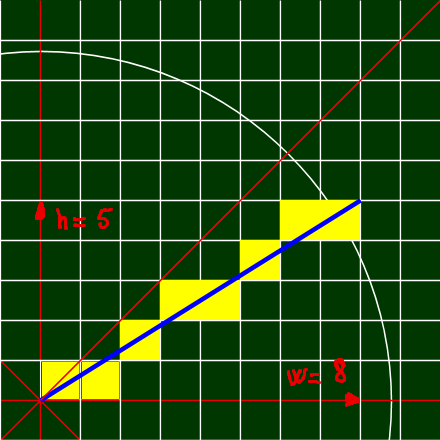
\includegraphics[width=0.35\textwidth]{imagenes/diario_desarrollo/linea_ideal.png}
\caption{Esquema algoritmo de Bresenham.}
\label{fig:bresenham}
\end{figure} 

Por otro lado, se añadieron herramientas para debug del movimientos de las entidades y las
diferentes componentes de este, para el dibujado de los vectores se eligió el algoritmo de
`\citeauthor*{Bresenham1962}', ya que, nos permite dibujar rectas de una forma efectiva
y sin consumir muchos recursos. Además, el algoritmo esta diseñado para trabajar con enteros,
cosa que hacemos a lo largo de todo el prototipo. En el esquema~\ref{fig:bresenham} la 
cuadricula blanca representa los pixeles de la plantalla, en color azul la recta ideal que
se busca dibujar y en amarillo la recta resultante del algoritmo.

Otra de las herramientas destinadas a poder análizar el funcionamiento del programa es
el control del tiempo de ejecución y el tamaño del \textit{`DeltaTime'}. Al poder disminuir
el número de fotogramas por segundo, podemos visualizar más detenidamente que sucede en
pantalla y ver que todo va según la previsión, por otra parte se puede aumentar la velocidad
para llegar antes a un punto de la ejecución en concreto. Además, jugar con el tamaño del
\textit{`DeltaTime'} nos permite experimentar con los valores de velocidad y/o otros factores
interpolados para ajustarlos de forma visual. 

Por último en cuanto a implementación, toda la información relacionada con el sistema de 
dibujado y los elementos visuales del juego se trabajan con \textit{uint64\_t}, mientras que
todo lo relacionado con el movimiento y demás calculos físicos se trabajan con
\textit{fint\_t\textless int64\_t\textgreater}. Por ello es necesario usar \textit{``casts``}
sobre los datos físicos con los que se quiera operar en el \textit{Render System}
\footnote{Ya sea la posición en el mapa como el sistema de debug para los vectores de
\textit{Steer}.}, como es una operación recurrente en el código se implementó un sistema 
auxiliar para convertir coordenada continuas (usadas en la mayoría de sistemas) a coordenadas de 
pantalla o pixel. 

\begin{figure}[ht]
\centering
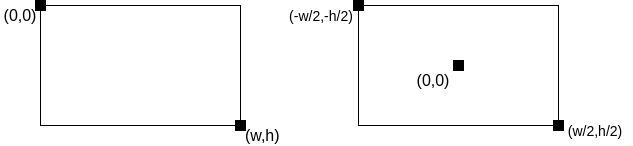
\includegraphics[width=0.8\textwidth]{imagenes/diario_desarrollo/sis_coords.png}\\
\hspace{-8mm} Coordenadas de pantalla. \hspace{16mm}  Coordenadas continuas.
\label{fig:sis_coords}
\end{figure} 

En lo referente a la memoria comenzamos la redacción de una versión preliminar del \ac{GDD}
donde comenzamos a describir las características del producto, del Estado del Arte donde se hace
mención a juegos que nos han servido de inspiración o modelo para imitar y se incluye una explicación
sobre las ténicas y algotimos se van a usar, y la explicación sobre la metodología seguida durante
este desarollo. 

\newpage

\section{Fase 1: Producto mínimo viable}
\begin{longtable}[c]{|p{7cm}|c|c|}
\hline
Iteraciones                                               & \% Completado & Termindo en \\ 
\hline
\endhead
\textbf{3.1.} Cambios en el motor ECS.                     & 100\% &   \\
	\cmidrule[.003pt]{1-3}
\textbf{3.2.} Cambios en el almacenamiento de datos.       & 100\% &   \\ 
	\cmidrule[.003pt]{1-3}
\textbf{3.3.} Cambio tipos propios a template.             & 100\% &   \\ 
	\cmidrule[.003pt]{1-3}
\textbf{3.4.} Cambio en el sistema de clases.              & 100\% &   \\
	
	\cmidrule[1pt]{1-3}

\textbf{4.1.} Añadir referente que use 
				\textit{Steering Behavior}.                & 100\% &   \\
	\cmidrule[.003pt]{1-3}
\textbf{4.2.} Diagrama y explicación de las fases de 
				una iteración.                             & 100\% &   \\
	\cmidrule[.003pt]{1-3}
\textbf{4.3.} Agrupar iteración en fases y describir el
				desarrollo hasta la fecha.                 & 30\%  &  It.5 \\
	\cmidrule[.003pt]{1-3}
\textbf{4.4.} Implementar mínimo producto.                 & 85\%  &  It.6 \\
	\cmidrule[.003pt]{1-3}
\textbf{4.5.} Análisis de resultados del MVP.              & 10\%  &  It.7 \\
	
	\cmidrule[1pt]{1-3}
	
\textbf{5.1.} Crear unidad de ataque a distancia.          & 100\% &   \\
	\cmidrule[.003pt]{1-3}
\textbf{5.2.} Adición de formación en anillo.              & 80\%  &  It.6 \\ 
	\cmidrule[.003pt]{1-3}
\textbf{5.3.} Balanceo de las unidades.                    & 0\%   &  It.8 \\ 
	\cmidrule[.003pt]{1-3}		
\textbf{5.4.} Profundizar los objetivos en el GDD y 
				explicar método de balanceo.               & 0\%   &  It.8 \\ 
	\cmidrule[.003pt]{1-3}		
\textbf{5.5.} Incluir tabla resumen al inicio de fase
				e incluir información extra como el set-up.& 100\%  &  \\

	\cmidrule[1pt]{1-3}

\textbf{6.1.} Experimentar con la formación en anillo
				y fuerzas cuadráticas.                     & 100\% &   \\
	\cmidrule[.003pt]{1-3}
\textbf{6.2.} Sistema de proyectiles para terminar la
				unidad a distancia.                        & 100\% &   \\
	\cmidrule[.003pt]{1-3}
\textbf{6.3.} Remplazar  TinyPTC por Dear ImGUI y
				hacer una interfaz básica.                 & 100\% &   \\
	\cmidrule[.003pt]{1-3}
\textbf{6.4.} Ajustar y continuar con la memoria.          & 80\%  & $\infty$ \\
	\cmidrule[.003pt]{1-3}
\textbf{6.5.} Profundizar en el GDD y listar cuestiones
				tecnológicas que hacen falta.              & 100\% &   \\
\hline
\caption{Resumen fase 1}
\end{longtable}

\subsection*{Iteración 3: Motor ECS y gestión de memoria}
La fase comenzó con una iteración corta debido a las vacaciones de Navidad y final de año, en la
que el foco estuvo despositado en refactorizar y dejar en mejor estado el código desarrollado
hasta el momento, donde se separó el nucleo principal del motor \ac{ECS} del conjunto de sistemas y
herramientas en dos \textit{namespaces} diferentes. 

Por el lado del motor \ac{ECS}, en un primer lugar el almacén de componentes estaba diseñado
para contener punteros a componentes, esto implicaba que los datos de los componentes se
guardaban en la memoria libre de forma ``anárquica''~\ref{fig:memoria_ptr}, 
en su lugar, lo deseado es almacenar todas las componentes de forma contigua para poder utilizar
la caché cuando sea posible, para poder aprovechar que es más rápida y minimizar la cantidad de
veces que mandamos al sistema ir a buscar nuestros datos~\ref{fig:memoria_obj}.

\begin{figure}[htb]
\centering
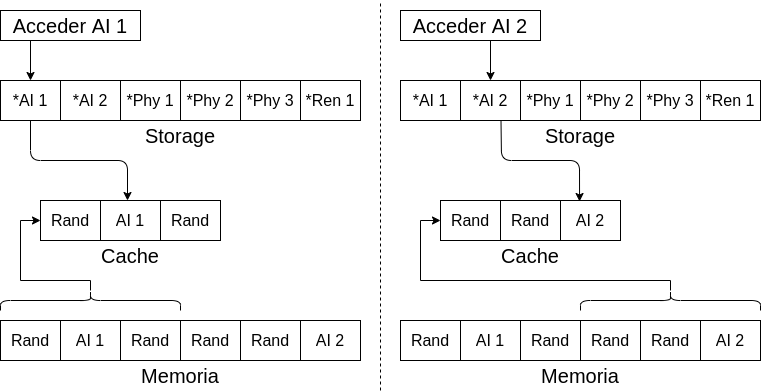
\includegraphics[width=0.7\textwidth]{imagenes/diario_desarrollo/memoria2.png}\\
\caption{Esquema acceso a vector de punteros.}
\label{fig:memoria_ptr}
\end{figure}

\begin{figure}[hbt]
\centering
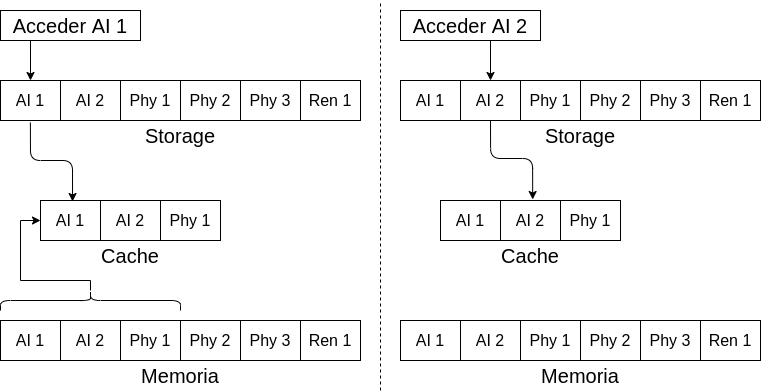
\includegraphics[width=0.7\textwidth]{imagenes/diario_desarrollo/memoria1.png}\\
\caption{Esquema acceso a vector de objetos.}
\label{fig:memoria_obj}
\end{figure}

A continuación, se modificó la estructura de las entidades para componerse unicamente de su
\textit{Entity ID} y una serie de \textit{Component ID}s para posibles comprobaciones de que
componentes contiene la entidad, dejando así de tener un puntero a las componentes del almacén.
Esto implica una serie de cambios en la fachada y uso del \textit{Entity manager} a la hora
de crear/eliminar entidades y la obtención de las componentes desde los sistemas a través del
contexto. 

Por último se siguieron modificando los tipos propios, tanto el \textit{fint\_t} como
los \textit{vec2} y \textit{fvec2} para trabajar como plantillas, pudiendo así librarnos de
la necesidad de crear un tipo completo para cada tipo básico con el que queramos usarlos.

\subsection*{Iteración 4: Combate, victoria y derrota}
Durante el mes de enero se implementaron diversas funcionalidades, en primer lugar abordamos
el sistema de combate del juego, para ello se creó una componente para almacenar elementos como
la vida de la unidad, su daño, el rango y el tiempo entre ataques, además, los sistemas de 
ataque para ir restando vida a las unidades conforme reciban daño, el de \textit{cooldown} para
actualizar los temporizadores para volver a atacar, y por último el sistema de muertes donde se
manda a pedir que se borren las entidades que hayan muerto y se realizan las comprobaciones 
de victoria y derrota de la partida.

Una vez se resuelve la partida, en el bucle de ejecución del juego se reiniciarán el nivel
vaciando y volviendo a cargar los elementos del juego.

Para incluir los nuevos sistemas y funcionalidades a la rutina de las unidades, se ha ampliado
el apartado de toma de decisión incluyendo métodos para detectar si hay unidades enemigas 
cerca y seleccionar como objetivo a la más cercana, que en caso de morir se lanzará una nueva
búsqueda. De forma similar, cuando no haya unidades enemigas cercanas se regresará al estado de
patrulla (en caso de la IA) y las manejadas por el jugador volveran a la posición de su
marcador en el mapa. 

En cuanto a la gestión de las unidades en partida, se creó un manejador de equipos donde se gestiona que
unidades pertenecen a cada facción, y proporcionar métodos para obtener los \textit{ID}s de las
unidades por equipo e ir actualizando los equipos cuanda haya bajas. Además de, tener métodos
para crear tipos de unidades en concreto trabajando a la vez de ``fábrica''.

Por otro lado, en el apartado visual, se ha añadido un marcador que indica la dirección a la
que se esta orientando la entidad con el fin de dar \textit{feedback} al jugador y que se 
entienda mejor y de forma visual el desplazamiento o acción actual. Este marcador tiene un 
tamaño relativo al del sprite de la unidad y serán siempre de color blanco para que sea
fácil de identificar. 

\begin{figure}[ht]
\centering
\begin{minipage}[c]{0.42\linewidth}
	\hspace{9mm}
	
\includegraphics[width=0.7\textwidth]{imagenes/diario_desarrollo/sin-marcador.png} \\
	\label{sin_marcador}
\end{minipage}
\begin{minipage}[c]{0.40\linewidth}
	\hspace{9mm}
	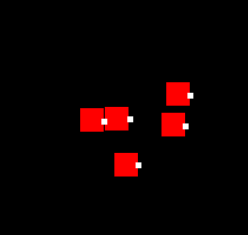
\includegraphics[width=0.7\textwidth]{imagenes/diario_desarrollo/marcador.png} \\
	\label{marcador}
\end{minipage} \\
	\hspace{0.5cm} Sin marcador. \hspace{3.5cm} Con marcador. 
\caption{Marcador dirección entidad.}
\end{figure}

Por último, en cuanto a la memoria, se ha añadido en el apartado de metodologia la
descripción de las fases que componen una iteración junto a un esquema. Se ha introducido
un tercer referente el cual basa toda su jugabilidad alrededor de los \textit{Steering
behavior}, debido a este juego hemos optado por cambiar la jugabilidad del proyecto
con el fin de imitar la de este juego y con intención de innovar en los controles, como ya se
refleja en el \ac{GDD}, actualmente el jugador no maneja directamente a las unidades con el
ratón ni las selecciona de forma individual, sino que controla un marcador verde el cual será
seguido por sus tropas y mediante ordenenes activará los distintos comportamientos de sus 
unidades. 

\subsection*{Iteración 5: Mecánicas fallidas}
A lo largo de la siguiente iteración se trabajó sobretodo en las mecánicas de juego, con el fin
de acercarse un poco más a la obtención de un prototipo que cumpla con los requisitos del \acs{MVP},
en concreto se comenzó el desarollo de un segundo tipo de unidad basada en ataques a distancia y 
la posibilidad de controlar la formación que siguen nuestras unidades, pudiendo alternar entre un
movimiento sin orden o una formación en anillo.

En cuanto a la unidad a distancia, gracias a que tenemos la componente de combate podemos ajustar de una
forma muy sencilla el rango de ataque de cada unidad, dejándonos la creación de un sistema de proyectiles
como tarea para completar el funcionamiento de dicha unidad. 

Por otro lado encontramos la formación en anillo, la cual cuenta con una primera versión que se basa en
modificar el rango de cohesión al centro del grupo en función de la distacia de ataque. Probando esta forma 
de configurar la posición de las unidades nos hemos dado cuenta de que no muestras buenos resultados en
conjuntos grandes de unidades, ya que, numerosas unidades quedan atrapadas en posiciones incorrectas y la
distribución resultante no es muy optima.

\begin{figure}[htb]
\centering
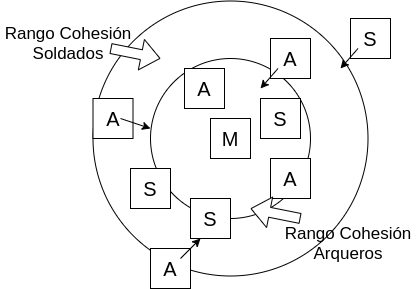
\includegraphics[width=0.45\textwidth]{imagenes/diario_desarrollo/anillo1.png}\\
\caption{Formación anillo por rango de cohesión}
\label{fig:anillo1}
\end{figure}

Por último, se ha introducido en la memoria una lista con las herramientas que han sido utilizadas 
durante el desarrollo, donde se incluye el nombre de las librerías, la versión y los sistemas sobre los que
puede ser lanzado el juego. Todo con el fin de ayudar a quién quiera utilizar, recompilar y/o 
modificar el prototipo. Además, se ha añadido al comienzo de cada fase una tabla resumen donde se indican
las tareas principales de cada iteración, el portentaje estimado de completado y, en caso de no haber sido
terminada, la iteración donde se ha finalizado.


\subsection*{Iteración 6: Interfaz y Dear ImGUI}
En la cuarta y última iteración de esta fase, el objetivo es el de terminar todas las mecánicas del prototipo
y sustituir \textit{\textless TinyPTC\textgreater} por \textit{\textless Dear ImGUI\textgreater} para poder
centrarnos más adelante en el diseño del nivel/es del prototipo de cara a la entrega final. Además de, poder
añadir alguna funcionalidad extra si es necesario para crear una experiencia de juego mejor.

Llegados a este punto, queremos crear una interfaz y tener la posibilidad de poder añadir algún elemento
visual al proyecto, por lo que necesitamos de una libreria que ofreza más opciones a la hora de trabajar
con ella. En este caso hemos elegido \textit{\textless Dear ImGUI\textgreater}
de \citeauthor*{dearimgui2021}, la cual, propone una nueva
forma de trabajar las interfaces\footnote{\textit{IMGUI (Immediate Mode GUI) paradigm.}} en auge actualmente
y además, nos proporciona una serie de \textit{widgets} y herramientas predefinidas que nos permitirán crear 
un HUD fácil y sencillo.
Además, funciona con \textit{GLFW} y \textit{OpenGL} así que si necesitamos revisar el funcionamiento de
alguna funcionalidad, no tendremos excesivos problemas ya que hemos trabajado con ellas anteriormente.


Para comenzar a trastear con esta librería, hemos implementado una pequeña ventana que nos permitirá manejar
en tiempo real el número de veces que se ejecutará el bucle del juego por segundo y/o el tamaño del 
\textit{DeltaTime}, además tiene un \textit{checkbox} para activar el debug visual del movimiento de las
entidades.

\begin{figure}[htb]
\centering
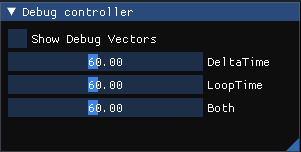
\includegraphics[width=0.45\textwidth]{imagenes/diario_desarrollo/hudDebug.png}\\
\caption{Herramienta depuración en tiempo de ejecución}
\label{fig:hudDebug}
\end{figure}

Por otro lado, se ha creado una segunda ventana que hará de "minimapa" y mostrará la ubícación de los unidades
tanto aliadas como enemigas y el marcador. Esto nos puede servir de cara a una versión del juego en el que el
mapeado sea más grande que la pantalla, para que nos permita visualizar y ubicarnos en el nivel.

\begin{figure}[htb]
\centering
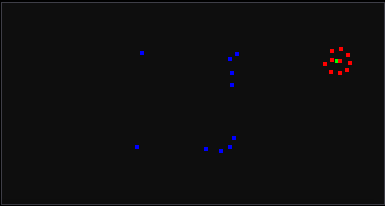
\includegraphics[width=0.45\textwidth]{imagenes/diario_desarrollo/minimap.png}\\
\caption{Mini Mapa.}
\label{fig:minimap}
\end{figure}

En cuanto a las mecánicas del juego, hemos añadido un sistema de lanzamiento de proyectiles para las unidades
que ataquen a distacia, esto incluye: la creación de las balas siguiendo la orientación del personaje, la
destrucción de las proyectiles una vez alcanzan su distancia máxima y/o impactan contra un objetivo.
La creación y destrucción de entidades se realiza al final del bucle del juego, al igual que con las
demás entidades. 

Un proyectil consiste en una entidad formada por una componente física para su desplazamiento, una para el
calculo de colisiones, y una visual para poder dibujarla. Una vez se lance un proyectil, este seguirá la
dirección que tenía la unidad al momento de disparar, por lo que solo hará daño si la unidad enemiga no 
cambia de posición lo suficiente para esquivar el área de impacto. A la hora de programar las colisiones,
solamente contaremos las unidades del bando contrario para optimizar el número de comprobaciones, para ello
tendrémos un vector de proyectiles por cada bando.

\begin{figure}[htb]
\centering
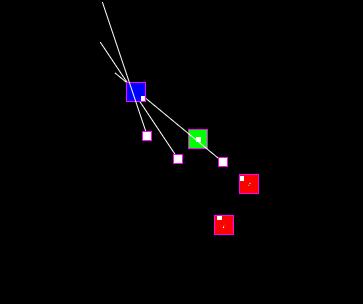
\includegraphics[width=0.45\textwidth]{imagenes/diario_desarrollo/balas.png}\\
\caption{Demostración sistema de disparos.}
\label{fig:balas}
\end{figure}

Otra de las mecánicas que han sido mejoradas, es la formación en anillo de nuestras unidades. Los resultados
y la forma generada eran poco satisfactorios por lo que se cambió de trabajar con la intensidad de la cohesión
a calcular una posición deseada para cada unidad en relación a su distancia de ataque. Para ello, mediante el
trazado de rayos creamos una recta entre el marcador del jugador y cada una de las distintas unidades, sobre esa
recta se marcará un punto el cual deberá ser alcanzado por la unidad, de esta forma solventamos los solapes entre
unidades y que se queden encerradas en lugares encorrectos, además de ser más escalable en caso de adición de
nuevas unidades en el futuro.

\begin{figure}[ht]
\centering
\begin{minipage}[c]{0.42\linewidth}
	\hspace{9mm}
	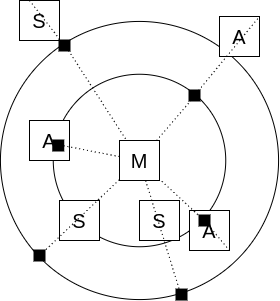
\includegraphics[width=0.7\textwidth]{imagenes/diario_desarrollo/anillo2.png} \\
	\label{anillo2}
\end{minipage}
\begin{minipage}[c]{0.42\linewidth}
	\hspace{9mm}
	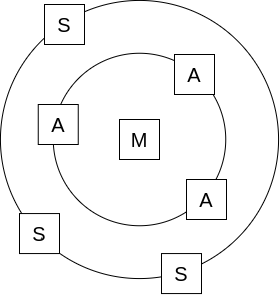
\includegraphics[width=0.7\textwidth]{imagenes/diario_desarrollo/anillo3.png} \\
	\label{anillo3}
\end{minipage}
\caption{Formación anillo con trazado de rayos.}
\end{figure}

Por último se ha cambiado el cálculo de las fuerzas de cohesión y separación para que tenga un crecimiento
cuadrático en lugar de lineal, de esta forma reducimos su presencia en la media/larga distacia y la aumentamos
en las cercanías.   

\begin{longtable}[c]{|c|c|c|}
\hline
Distancia & Lineal  & Cuadrado \\
\hline
\endhead
40  & \multicolumn{1}{S|}{5.59}   & \multicolumn{1}{S|}{31.25}  \\
\cmidrule[0.15pt]{0-2}
60  & \multicolumn{1}{S|}{2.484}  & \multicolumn{1}{S|}{6.1728} \\ 
\cmidrule[0.15pt]{0-2}
80  & \multicolumn{1}{S|}{1.3975} & \multicolumn{1}{S|}{1.953}  \\ 
\cmidrule[0.15pt]{0-2}
100 & \multicolumn{1}{S|}{0.8944} & \multicolumn{1}{S|}{0.8}    \\
\cmidrule[0.15pt]{0-2}
120 & \multicolumn{1}{S|}{0.621}  & \multicolumn{1}{S|}{0.3858} \\
\cmidrule[0.15pt]{0-2}
140 & \multicolumn{1}{S|}{0.4563} & \multicolumn{1}{S|}{0.2082} \\
\cmidrule[0.15pt]{0-2}
160 & \multicolumn{1}{S|}{0.3494} & \multicolumn{1}{S|}{0.1221} \\
\cmidrule[0.15pt]{0-2}
180 & \multicolumn{1}{S|}{0.2760} & \multicolumn{1}{S|}{0.0762} \\
\cmidrule[0.15pt]{0-2}
200 & \multicolumn{1}{S|}{0.2236} & \multicolumn{1}{S|}{0.05}   \\
\cmidrule[0.15pt]{0-2}
220 & \multicolumn{1}{S|}{0.1848} & \multicolumn{1}{S|}{0.0342} \\
\hline
\caption{Fuerzas de separación en función de la distancia}
\end{longtable}

\newpage

\section{Fase 2: Últimos pasos}
\begin{longtable}[c]{|p{7cm}|c|c|}
\hline
Iteraciones                                                & \% Completado & Termindo en \\ 
\hline
\endhead
\textbf{7.1.} Continuar trabajando el GDD.                 & 10\% & It.X  \\
	\cmidrule[.003pt]{1-3}
\textbf{7.2.} Ajustes de valores de daño y vida.           &  0\% & It.X  \\ 
	\cmidrule[.003pt]{1-3}
\textbf{7.3.} Incluir los ciclos de análisis de los 
				comportamientos resultantes y 
				propuestas de mejora                       & 40\% & It.X  \\ 
	\cmidrule[.003pt]{1-3}
\textbf{7.4.} Revisar bugs y comportamientos erróneos.     & 100\% & \\
	\cmidrule[.003pt]{1-3}
\textbf{7.5.} Incluir sistema de cámara y coordenadas 
				de mundo.                                  & 100\% & \\
	\cmidrule[.003pt]{1-3}
\textbf{7.6.} Implementar jugabilidad básica: debe poder
				jugarse una partida simple al juego, con
				las reglas propuestas.                     & \% & It.X  \\

		\cmidrule[1pt]{1-3}

\textbf{8.1.} Balanceo de unidades y ajustar sus valores.  & \% &  \\
	\cmidrule[.003pt]{1-3}
\textbf{8.2.} Redactar de forma detallada el balanceo.     & \% &  \\
	\cmidrule[.003pt]{1-3}
\textbf{8.3.} Prueba de compilación cruzada para Windows.  & \% &  \\
	\cmidrule[.003pt]{1-3}
\textbf{8.4.} Describir todas las herramientas implementadas
				y procesos de analasis.                    & \% &  \\
\hline
\caption{Resumen fase 3}
\end{longtable}

\subsection*{Iteración 7: Terminando las cuestiones tecnológicas}
A lo largo de esta iteración los objetivos propuestos eran los de terminar de implementar y/o corregir
las mecánicas y sistemas del proyecto, a la vez que se continua en la redacción de la memoria y el GDD.
De esta forma poder dejar las ultimas iteraciones en diseñar los niveles, balancear el juego y terminar
de redactar la memoria.

Uno de los puntos principales cae sobre la resolución de un error en las colisiones de las balas,
este problema consistía en una serie de balas que atravesaban a las unidades con baja frecuencía
y sin motivo aparente. Con el fin de subsanar este problema se ha creado una componente de colisiones
la cual ha sustituido el uso del tamaño del sprite en los calculos de colisiones con el límite de la 
ventana y demás entidades. \\
Al integrar esta componente en el sistema de debug visual pudimos observar como el problema era que las
colisiones estan siendo calculadas teniendo en cuenta el centro de la entidad, cuando el origen de ésta
es la esquina superior izquierda, esto suponía un desplazamiento de todas las colisiones y por lo tanto
errores en las detección, con cambiar ese factor se solucionaron todos los problemas.

A lo largo de la ejecución del programa, podíamos ver como algunas unidades se quedaban quietas sin poder
retomar su movimiento hasta que otra unidad la desplazaba y hacía reaccionar, después de analizar la situación
pudimos determinar que el problema ocurría cuando la unidad perdía su velocidad y aceleración dentro del
rango de ``velocidad reducida'' del \textit{`Arrive behaviour'}, lo que estaba sucediendo, es que no se
estaban calculando correctamente las divisiones con enteros de coma fija cuyo resultado era un valor
entre 0 y 1.

\begin{figure}[ht]
\centering
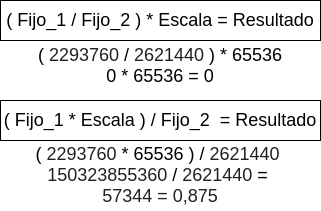
\includegraphics[width=0.45\textwidth]{imagenes/diario_desarrollo/division_entera.png}\\
\caption{Comparación resultados división.}
\label{fig:div_int}
\end{figure}

En una primera versión del operador, el cálculo que se realizaba era: dividir primero los valores a operar
y después multiplicar el resultado por la `Escala', este orden de los factores nos llevaba a que si, en la
primera operación el divisor era mayor que el dividendo, el valor del resto era 0, ya que trabajamos
con enteros y trunca los valores decimales.

Para solucionar el problema, lo que se hizo fue extraer una versión reducida del tipo de dato que sólo contaba
con las operaciones de división e introducirla en `Godbolt'\footnote{\url{https://godbolt.org}}, para poder
realizar una serie de pruebas y ajustes rápidamente sin tener que estar pendiente del resto del proyecto. \\
Una vez teníamos ya las funciones listas, lo único que quedaba era experimentar con el orden de los
factores a la hora de realizar la operación y ver si el resultado variaba. Tras un ligero ajuste conseguimos
que la operación conservara el valor deseado, esto se logró multiplicando el primer valor de la operación
por la `Escala' antes de dividir por el segundo dígito, de esta forma evitamos los resultados entre 0 y 65536
y que se trunque el valor en mitad de la operación.

Una vez solventados los errores, nos pusimos a crear lo necesario para poder diseñar niveles más amplios,
para ello incluímos un sistema de cámaras, el cual mostrará la porción del nivel donde se encuentre
nuestro puntero y unidades, el seguimiento se hace utilizando el \textit{`Arrive behaviour'} de forma que
el movimiento de la cámara comienza cuando nos separamos una cierta distancia del centro de la escena.

\begin{figure}[ht]
\centering
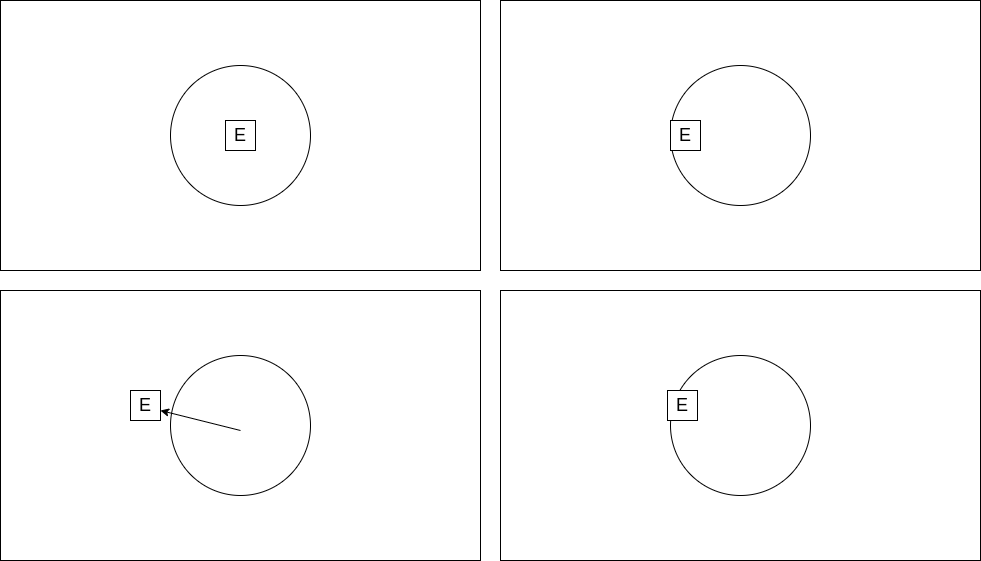
\includegraphics[width=0.6\textwidth]{imagenes/diario_desarrollo/camara.png}\\
\caption{Arrive behaviour en la cámara}
\label{fig:arrive_cam}
\end{figure}

Ahora las dimensiones de la pantalla pasan a ser las de la cámara y el nivel tendrá unas dimensiones
propias, las cuales usaremos para limitar el movimiento de las unidades, por lo que las unidades se pueden
mover libremente fuera de nuestro campo de visión siempre y cuando estén en los límites del nivel,
mientras estén fuera de cámara solo se dibujaran en el minimapa para evitar hacer llamadas inútiles. \\
Además de los cálculos para las colisiones, otro requisito fue adaptar el minimapa para que mostrara
que parte del nivel esta siendo visualizado y que nos permita úbicar a todas las unidades y objetivos
fuera de cámara. Un detalle importante es que al crear el nivel, le indicamos al motor la relación
entre las dimensiones de pantalla y nivel, por lo que los objetos mostrados en el minimapa se ajustarán
en función de este parámetro, cuanto más grande el nivel, más pequeños serán los elementos.

\begin{figure}[ht]
\centering
\includegraphics[width=0.6\textwidth]{imagenes/diario_desarrollo/minimap2.png}\\
\caption{Cambios en el minimapa}
\label{fig:minimap2}
\end{figure}

En lo referente al \textit{HUD}, se ha añadido también un selector de comportamiento y formación
para nuestras unidades, de esta forma podremos controlar dichos parametros con simples \textit{clicks}
y ahorrarnos el tener que disponer de una tecla para cada opción. 

\begin{figure}[ht]
\centering
\includegraphics[width=0.45\textwidth]{imagenes/diario_desarrollo/eleccion_b.png}\\
\caption{Selector de comportamiento y formación}
\label{fig:hud_selec}
\end{figure}

En lo referente a la mecánicas y comportamientos de las entidades han habido dos cambios relevantes durante
la iteración, en primer lugar encontramos la adición de un componente \textit{singleton} de \textit{Blackboard}
el cual nos permitirá almacenar información compartida para todas las unidades bajo nuestro control, además de
controlar la frecuencia en la que la esta información se actualiza, esto nos permitirá crear una sensación
de retraso en la reacción a nuestras acciones por parte de las unidades a la vez que nos permite eliminar
la necesidad de guardar la misma información en cada componente de \ac{IA} por unidad que tengamos.

En segundo lugar encontramos otro cambio en las componentes de \ac{IA}, esta vez con efectos sobre las unidades
controladas por la máquina, en este caso se trata de la creación de una estructura auxiliar que representa 
y contiene las rutas que las unidades seguirán mientras no estén peleando contra nosotros.

En un inicio estas rutas se encontraban directamente en la componente, actualmente en la componente podemos
encontrar un ``iterador de ruta'' el cual nos podrá facilitar la siguiente posición y gestionar como avanzamos
por la patrulla, de forma que si llegamos al final de forma automática nos devolverá la primera posición
que recorrimos. De esta forma evitamos errores en la gestión de las patrullas y dublicar la información de estas.
 

\subsection*{Iteración 8: Diseño de niveles}
Durante esta penúltima iteración buscamos conseguir un prototipo que ofrezca una experiencia
de juego capaz de mostrar todas las herramientas diseñadas y entretener al jugador. Para ello se han 
planteado objetivos relacionados con el diseño de los niveles y el balanceo de las unidades, tratando
de conseguir el que el jugador sepa en todo momento su objetivo en el juego y que sea atractivo para el.

En primer lugar hemos trabajado el balanceo de los valores de vida y daño de los distintos tipos de
unidades, partiendo de una situación con todas las unidades con los mismos valores
debemos tratar de darles ventajas y desventajas a cada una de ellas, con el fin de obligar al
jugador a pensar bien como colocarlas y utilizarlas. Durante el proceso se ha desarrollado un excel
para observar los valores y modificarlos de forma rápida, esto nos ayuda a poder hacer un análisis
profundo de los efectos de cada valor en el resultado de las unidades.

\begin{longtable}[c]{|c|c|c|c|c|c|}
\hline
\multicolumn{1}{|m{1.8cm}|}{Tiempo de refresco} & \multicolumn{1}{m{1.2cm}|}{Ataque}             &
\multicolumn{1}{m{1.7cm}|}{Daño por segundo}   & \multicolumn{1}{m{1.4cm}|}{Vida enemiga}        &
\multicolumn{1}{m{1.2cm}|}{Tiempo para matar}  & \multicolumn{1}{m{1.45cm}|}{Impactos para matar}\\
\hline
\hline
\endhead
\multicolumn{1}{|S|}{2} & \multicolumn{1}{S|}{4} & \multicolumn{1}{S|}{2} & 
\multicolumn{1}{S|}{12} & \multicolumn{1}{S|}{6} & \multicolumn{1}{S|}{3} \\
\hline
\multicolumn{1}{|S|}{2} & \multicolumn{1}{S|}{4} & \multicolumn{1}{S|}{2}   & 
\multicolumn{1}{S|}{14} & \multicolumn{1}{S|}{7} & \multicolumn{1}{S|}{3.5} \\ 
\hline
\multicolumn{1}{|S|}{2} & \multicolumn{1}{S|}{5}   & \multicolumn{1}{S|}{2.5} & 
\multicolumn{1}{S|}{12} & \multicolumn{1}{S|}{4.8} & \multicolumn{1}{S|}{2.4} \\ 
\hline
\multicolumn{1}{|S|}{2} & \multicolumn{1}{S|}{5}   & \multicolumn{1}{S|}{2.5} & 
\multicolumn{1}{S|}{14} & \multicolumn{1}{S|}{5.6} & \multicolumn{1}{S|}{2.8} \\
\hline
\multicolumn{1}{|S|}{3} & \multicolumn{1}{S|}{5}   & \multicolumn{1}{S|}{1.667} & 
\multicolumn{1}{S|}{12} & \multicolumn{1}{S|}{7.2} & \multicolumn{1}{S|}{2.4}   \\
\hline
\multicolumn{1}{|S|}{3} & \multicolumn{1}{S|}{5}   & \multicolumn{1}{S|}{1.667} & 
\multicolumn{1}{S|}{14} & \multicolumn{1}{S|}{8.4} & \multicolumn{1}{S|}{2.8}   \\
\hline
\caption{Valores arquero vs soldado}
\end{longtable}

La idea es lograr que el jugador sienta que los Soldados son unidades más resistentes pero con menor
daño, para ello les dotaremos de mayor vida pero menor daño que a los arqueros, por otro lado, realizar
un movimiento con las manos es una acción que requiere mucha menos preparación y dedicación que cargar 
un arco, por ello se contempla darles una mayor frecuencia a sus ataques.

\begin{longtable}[c]{|c|c|c|c|c|c|}
\hline
\multicolumn{1}{|m{1.8cm}|}{Tiempo de refresco} & \multicolumn{1}{m{1.2cm}|}{Ataque}             &
\multicolumn{1}{m{1.7cm}|}{Daño por segundo}   & \multicolumn{1}{m{1.4cm}|}{Vida enemiga}        &
\multicolumn{1}{m{1.2cm}|}{Tiempo para matar}  & \multicolumn{1}{m{1.45cm}|}{Impactos para matar}\\
\hline
\hline
\endhead
\multicolumn{1}{|S|}{2} & \multicolumn{1}{S|}{4} & \multicolumn{1}{S|}{2} & 
\multicolumn{1}{S|}{6}  & \multicolumn{1}{S|}{3} & \multicolumn{1}{S|}{1.5} \\
\hline
\multicolumn{1}{|S|}{2} & \multicolumn{1}{S|}{4} & \multicolumn{1}{S|}{2}   & 
\multicolumn{1}{S|}{8}  & \multicolumn{1}{S|}{4} & \multicolumn{1}{S|}{2} \\ 
\hline
\multicolumn{1}{|S|}{2} & \multicolumn{1}{S|}{5}   & \multicolumn{1}{S|}{2.5} & 
\multicolumn{1}{S|}{6}  & \multicolumn{1}{S|}{2.4} & \multicolumn{1}{S|}{1.2} \\ 
\hline
\multicolumn{1}{|S|}{2} & \multicolumn{1}{S|}{5}   & \multicolumn{1}{S|}{2.5} & 
\multicolumn{1}{S|}{8}  & \multicolumn{1}{S|}{3.2} & \multicolumn{1}{S|}{1.6} \\
\hline
\multicolumn{1}{|S|}{3} & \multicolumn{1}{S|}{5}   & \multicolumn{1}{S|}{1.667} & 
\multicolumn{1}{S|}{6}  & \multicolumn{1}{S|}{3.6} & \multicolumn{1}{S|}{1.2}   \\
\hline
\multicolumn{1}{|S|}{3} & \multicolumn{1}{S|}{5}   & \multicolumn{1}{S|}{1.667} & 
\multicolumn{1}{S|}{8}  & \multicolumn{1}{S|}{4.8} & \multicolumn{1}{S|}{1.6}   \\
\hline
\caption{Valores soldado vs arquero}
\end{longtable}

Los arqueros por su lado, están pensados como unidades de mediano alcance que atacan con proyectiles.
Son débiles y si tratan de avanzar solos podrían ser masacrados por grupos de soldados, para evitarlo 
el jugador deberá intentar proteger a sus arqueros utilizando a sus guerreros como muro defensivo. 
A pesar de que realizan más daño a sus rivales, los proyectiles no realizan un daño inmediato, sino que
actuan al impactar, cosa que podría no suceder. Esto nos ayuda a equilibrar la balanza debido a la ventaja
de rango que poseen los arqueros.

El segundo lugar encontramos el diseño de los niveles, a la hora de establecer la cantidad de enemigos
y su disposición tenemos que tener en cuenta el objetivo del nivel, si el nivel consiste en limpiar
todos los enemigos existentes tendremos que evaluar la cantidad y como se agrupan para que puedan
ser limpiados si gestionas medianamente bien las unidades. Si el objetivo es llegar a un punto en concreto
del nivel, los enemigos serán más y el combate directo nos pondrá en aprietos, por lo que el objetivo
debería ser encontrar una ruta que nos asegure el menor nivel de conflicto posible.

\subsection*{Iteración 9: Retoques y preparación entrega}

\placeholdertext{tiggers}
\placeholdertext{mensajes estaticos mapa}
\placeholdertext{complilación windows}

\placeholdertext{terminar de escribir memoria}
\placeholdertext{poster + docs entrega}



%input{capitulos/resultados}
%input{capitulos/conclusiones}

%\nocite{*} %incluye TODOS los documentos de la base de datos bibliográfica sean o no citados en el texto
\bibliography{bibliografia/bibliografia.bib}\addcontentsline{toc}{chapter}{Bibliografía} %sustituir bibliografía con el nombre del fichero bibtex con la bibliografía
\bibliographystyle{apalike}
%
%\appendix
%\chapter{Anexo I}
Aquí vendría en anexo I 

\end{document}
